\section{Chuỗi xử lý thời gian thực, tối ưu và xuất dữ liệu}

\subsection{Chuỗi xử lý thời gian thực và truyền phát dữ liệu}

\subsubsection{Kiến trúc chuỗi xử lý thời gian thực}

\hspace{0.5cm} Giai đoạn này tích hợp các thuật toán lọc Kalman và alpha-beta đã phát triển vào chuỗi xử lý thời gian thực từ cảm biến đến giao diện người dùng. Mục tiêu là đảm bảo dữ liệu bám mục tiêu được cập nhật liên tục với độ trễ tối thiểu, duy trì độ chính xác của các phép tính tọa độ và lọc. Toàn bộ chuỗi hoạt động liên tục ở tần số 10 Hz, mỗi chu kỳ tương đương 100 ms, trong đó toàn bộ dữ liệu được nhận, xử lý và hiển thị.

\subsubsection{Tổng quan luồng dữ liệu}

\hspace{0.5cm} Luồng dữ liệu trong hệ thống gồm hai nhánh song song: nhánh đo lường (measurement path) đưa dữ liệu thô từ cảm biến qua các bước xử lý để ước lượng vị trí mục tiêu, và nhánh điều khiển (control path) điều phối luồng dữ liệu, quản lý trạng thái phiên và phát kết quả đến giao diện. Hình \ref{fig:data-flow} mô tả toàn bộ chuỗi xử lý từ cảm biến đến giao diện.

\begin{figure}[H]
\centering
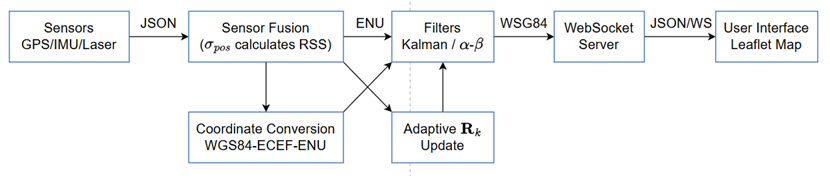
\includegraphics[width=0.9\textwidth]{Images/real-time-data-pipeline.png}
\caption{Chuỗi xử lý thời gian thực từ cảm biến đến giao diện}
\label{fig:data-flow}
\end{figure}

Mỗi chu kỳ 10 Hz, chuỗi xử lý gồm bảy bước, mỗi bước có ngân sách thời gian (timing budget) riêng được thiết kế để toàn bộ chu kỳ luôn nằm trong giới hạn 100 ms:

\begin{enumerate}
    \item \textbf{Nhận gói tin cảm biến:} Kênh truyền dữ liệu hai chiều nhận gói tin JSON từ thiết bị quan sát. Gói tin chứa tọa độ GPS, góc azimuth/elevation từ IMU và khoảng cách từ cảm biến laser. Ngân sách thời gian: 5 ms, bao gồm giải mã JSON và kiểm tra tính hợp lệ của các trường dữ liệu.

    \item \textbf{Tính $\sigma_{pos}$ và chuẩn hóa đo lường:} Sử dụng công thức lan truyền sai số dựa trên khoảng cách laser để tính độ bất định vị trí $\sigma_{pos}$. Công thức hồi quy đa thức bậc hai:\ $\sigma_{pos} = 4.088 - 0.0158 \cdot d + 0.0000427 \cdot d^2$, trong đó $d$ là khoảng cách laser (m). Ngân sách thời gian: 2 ms.

    \item \textbf{Chuyển đổi tọa độ LLA sang ENU:} Tọa độ WGS84 (vĩ độ, kinh độ, chiều cao) được chuyển sang hệ tọa độ Local Tangent Plane (ENU) với người quan sát làm gốc. Chuỗi chuyển đổi gồm hai bước: LLA$\to$ECEF sử dụng phép chiếu ellipsoid WGS84, sau đó ECEF$\to$ENU sử dụng ma trận xoay 3$\times$3. Ngân sách thời gian: 6 ms, trong đó 2 ms cho LLA$\to$ECEF và 3,8 ms cho ECEF$\to$ENU.

    \item \textbf{Hợp nhất cảm biến (Sensor Fusion):} Kết hợp khoảng cách laser với tọa độ GPS đã chuyển sang ENU để tạo ra vị trí hợp nhất. Phương pháp trọng số nghịch đảo khoảng cách (inverse-distance weighting) được sử dụng. Ngân sách thời gian: 1,2 ms.

    \item \textbf{Chạy bộ lọc (Kalman / Alpha-beta):} Bộ lọc Kalman chạy trên vector trạng thái 6 chiều (vị trí 3D + vận tốc 3D), thực hiện hai pha predict và update. Bộ lọc alpha-beta chạy trên mặt phẳng 2D với trạng thái 4 chiều (vị trí 2D + vận tốc 2D). Ngân sách thời gian: 48,5 ms, chiếm phần lớn chu kỳ do phép nhân và giải hệ phương trình tuyến tính.

    \item \textbf{Chuyển kết quả ngược về WGS84:} Vị trí ước lượng từ ENU được chuyển ngược về tọa độ WGS84 thông qua chuỗi nghịch đảo ENU$\to$ECEF$\to$LLA. Ngân sách thời gian: 3,4 ms.

    \item \textbf{Phát kết quả đến giao diện:} Gói tin JSON chứa vị trí ước lượng, độ bất định và số bước được gửi qua kênh truyền dữ liệu hai chiều đến giao diện người dùng. Ngân sách thời gian: 3 ms.
\end{enumerate}

Bảng \ref{tab:pipeline-timing-w12} tổng hợp ngân sách thời gian của toàn bộ chu kỳ xử lý.

Biên an toàn 31\% (tương đương 31 ms) đủ lớn để xử lý các biến động về thời gian thực thi, bao gồm giải phóng bộ nhớ của trình duyệt, tắc nghẽn mạng cục bộ, hoặc các tác vụ phụ trợ khác. Giới hạn thời gian thực (real-time constraint) đặt ra cho toàn bộ chuỗi là 100 ms, và chuỗi xử lý hiện tại đáp ứng thoải mái với biên dự phòng đáng kể.

\subsubsection{Kiến trúc module hóa}

\hspace{0.5cm} Chuỗi xử lý được thiết kế theo kiến trúc module hóa, mỗi bước xử lý là một hàm riêng biệt có đầu vào và đầu ra rõ ràng. Thiết kế này giúp kiểm tra đơn vị (unit testing) từng bước, thay đổi thuật toán lọc mà không ảnh hưởng đến các bước khác, và theo dõi thời gian thực thi từng bước để cải thiện hiệu năng. Ma trận trạng thái $\mathbf{x}_k$ và ma trận hiệp phương sai $\mathbf{P}_k$ của Kalman filter được truyền qua các bước mà không sao chép bộ nhớ, giảm thiểu overhead phân bổ bộ nhớ động.

\subsubsection{Thiết kế kênh truyền dữ liệu hai chiều}

\hspace{0.5cm} Kênh truyền dữ liệu hai chiều (WebSocket) được chọn làm giao thức truyền tải chính cho chuỗi xử lý thời gian thực. Lựa chọn này dựa trên phân tích so sánh ba phương án giao thức: HTTP polling, Server-Sent Events (SSE) và WebSocket. Mỗi phương án có ưu nhược riêng, nhưng chỉ WebSocket đáp ứng đầy đủ yêu cầu của bài toán bám mục tiêu thời gian thực.

\subsubsection{So sánh ba phương án giao thức}

\hspace{0.5cm} HTTP polling đòi hỏi máy khách gửi request định kỳ, mỗi request kèm header HTTP đầy đủ khoảng 500 byte, tạo overhead lớn khi chạy ở tần số cao. Server-Sent Events (SSE) cải thiện hơn với kết nối một chiều persistent, nhưng không hỗ trợ máy khách gửi dữ liệu cảm biến lên server. WebSocket thiết lập kết nối persistent hai chiều, cho phép cả hai phía chủ động gửi dữ liệu với độ trễ thấp nhất.

\subsubsection{Lý do lựa chọn WebSocket}

\hspace{0.5cm} Ba lý do chính dẫn đến lựa chọn WebSocket thay vì các phương án khác:

\begin{itemize}
    \item \textbf{Độ trễ thấp:} Ở tần số 10 Hz, mỗi chu kỳ xử lý là 100 ms. HTTP polling với độ trễ$\geq$ 1 chu kỳ sẽ chiếm toàn bộ thời gian xử lý chỉ cho việc truyền tải. WebSocket với độ trễ$\sim$3 ms để lại 97 ms cho xử lý thực tế.

    \item \textbf{Hai chiều đồng thời:} Máy khách cần gửi dữ liệu cảm biến (GPS, IMU, laser) lên server, đồng thời server phát kết quả lọc (vị trí ước lượng, độ bất định) xuống máy khách. WebSocket hỗ trợ full-duplex, cả hai phía có thể gửi dữ liệu bất cứ lúc nào mà không cần chờ phía kia phản hồi.

    \item \textbf{Overhead thấp:} Sau lần thiết lập kết nối ban đầu (handshake HTTP upgrade), WebSocket không kèm HTTP header ở mỗi frame dữ liệu, giảm overhead truyền tải đáng kể so với HTTP polling.
\end{itemize}

\subsubsection{Kênh truyền dữ liệu và proxy}

\hspace{0.5cm} Kênh truyền dữ liệu hai chiều được đặt tại đường dẫn riêng, tách biệt hoàn toàn khỏi các endpoint REST. Trong môi trường phát triển, giao diện React chạy trên máy khách được cấu hình proxy để chuyển tiếp các yêu cầu kênh truyền dữ liệu hai chiều đến server backend. Thiết kế proxy này giúp tránh các vấn đề liên quan đến chính sách chia sẻ nguồn gốc chéo (Cross-Origin Resource Sharing) trong quá trình phát triển, đồng thời đơn giản hóa cấu hình mạng khi triển khai production.

\subsubsection{Cấu trúc bản tin dữ liệu}

\hspace{0.5cm} Hệ thống sử dụng định dạng JSON chuẩn hóa cho tất cả các bản tin (message) truyền tải qua kênh truyền dữ liệu hai chiều. Mỗi bản tin có trường thời gian (timestamp) dưới dạng số có dấu phẩy động, biểu thị thời gian Unix tính bằng giây, cho phép đồng bộ thời gian giữa cảm biến, server và giao diện.

\subsubsection{Bản tin cảm biến (client \texorpdfstring{$\to$}{to} server)}

\hspace{0.5cm} Mỗi bản tin từ thiết bị quan sát lên server chứa ba nhóm dữ liệu cảm biến chính:

\begin{itemize}
    \item \textbf{GPS:} Tọa độ WGS84 gồm vĩ độ (degree), kinh độ (degree) và chiều cao (mét). Chiều cao được dùng khi mục tiêu bay ở độ cao (drone), còn người đi bộ và xe máy thường ở mức mặt đất.

    \item \textbf{IMU:} Góc ngang (azimuth, độ) và góc nâng (elevation, độ) từ cảm biến đo quán tính, xác định phương hướng quan sát từ người quan sát đến mục tiêu.

    \item \textbf{Laser:} Khoảng cách (mét) từ cảm biến laser đến mục tiêu, là nguồn thông tin khoảng cách chính xác nhất trong hệ thống.
\end{itemize}

Cấu trúc bản tin cảm biến gồm các trường sau:

\subsubsection{Bản tin kết quả (server \texorpdfstring{$\to$}{->} client)}

\hspace{0.5cm} Server phản hồi sau mỗi bước xử lý, bản tin chứa vị trí ước lượng từ cả hai bộ lọc và thông tin hỗ trợ hiển thị:

\begin{itemize}
    \item \textbf{target}: Vị trí ước lượng từ hợp nhất cảm biến (đã chuyển về WGS84), dùng làm lớp quỹ đạo thô (raw trajectory).

    \item \textbf{kalman}: Vị trí ước lượng từ bộ lọc Kalman, kèm bán kính bất định thể hiện mức tin cậy của ước lượng.

    \item \textbf{alphabeta}: Vị trí ước lượng từ bộ lọc alpha-beta, chỉ trên mặt phẳng East-North, không có chiều cao.

    \item \textbf{step}: Số thứ tự bước thời gian hiện tại, bắt đầu từ 0 mỗi phiên mới.
\end{itemize}

Cấu trúc bản tin kết quả gồm các trường sau:

Bán kính bất định được tính từ công thức $\sigma_{pos} = \sqrt{\operatorname{tr}(\mathbf{P}_k)/n}$, với $\operatorname{tr}$ là vết (trace) của ma trận hiệp phương sai $\mathbf{P}_k$ và $n$ là số chiều trạng thái. Giá trị này cho phép giao diện hiển thị vòng tròn bất định quanh ước lượng Kalman, phản ánh mức độ tin tưởng của bộ lọc vào ước lượng vị trí tại mỗi bước thời gian.

\subsubsection{Quản lý phiên làm việc}

\hspace{0.5cm} Mỗi lần bám mục tiêu được tổ chức thành một phiên (session) độc lập. Kiến trúc phiên này cho phép chạy nhiều phiên đồng thời nếu có nhiều thiết bị quan sát cùng lúc, và cô lập trạng thái bộ lọc giữa các phiên để tránh nhiễu chéo. Trạng thái của mỗi phiên bao gồm vector trạng thái $\mathbf{x}_k$, ma trận hiệp phương sai $\mathbf{P}_k$, bộ đệm quỹ đạo và số bước thời gian hiện tại.

\subsubsection{Vòng đời phiên}

\hspace{0.5cm} Bảng \ref{tab:server-session-lifecycle} mô tả bốn giai đoạn trong vòng đời của một phiên tracking.

\subsubsection{Lưu trữ trong bộ nhớ}

\hspace{0.5cm} Trạng thái bộ lọc (vector trạng thái $\mathbf{x}$, ma trận hiệp phương sai $\mathbf{P}$) được lưu trong bộ nhớ trong (in-memory storage) suốt vòng đời phiên. Điều này đảm bảo truy cập nhanh trong mỗi chu kỳ xử lý mà không cần đọc/ghi từ đĩa cứng. Khi phiên kết thúc hoặc kênh truyền dữ liệu hai chiều đóng, toàn bộ trạng thái được giải phóng ngay lập tức khỏi bộ nhớ, tránh rò rỉ bộ nhớ trong các phiên dài.

Bộ đệm quỹ đạo (trajectory buffer) của mỗi phiên cũng được lưu trong bộ nhớ, chứa lịch sử 500 điểm dữ liệu gần nhất. Tổng bộ nhớ mỗi phiên ước tính khoảng 50 KB, bao gồm 384 byte cho ma trận $\mathbf{P}$ (6$\times$6$\times$8 byte), 48 byte cho vector $\mathbf{x}$ (6$\times$8 byte) và khoảng 48 KB cho bộ đệm quỹ đạo (500 điểm $\times$ 3 lớp $\times$ 32 byte/điểm).

\subsubsection{Bộ đệm vòng tròn (Ring Buffer)}

\hspace{0.5cm} Giao diện lưu lịch sử quỹ đạo bằng vùng đệm vòng (ring buffer) với dung lượng cố định $N_{max} = 500$ điểm. Cấu trúc bộ nhớ này đảm bảo dung lượng không tăng không giới hạn trong các phiên làm việc kéo dài. Khi vùng đệm đầy, điểm dữ liệu cũ nhất bị ghi đè bởi điểm mới nhất theo nguyên tắc FIFO (First-In, First-Out):

\begin{equation}
\text{buffer}[k \bmod N_{max}] \leftarrow \mathbf{p}_{target,k}
\end{equation}

trong đó $k$ là chỉ số bước thời gian hiện tại và $\mathbf{p}_{target,k}$ là tọa độ mục tiêu tại bước $k$.

\subsubsection{Phân tích độ phức tạp}

\hspace{0.5cm} Bộ đệm vòng tròn có độ phức tạp thời gian $O(1)$ cho cả hai thao tác chèn và truy xuất, so với mảng thông thường có độ phức tạp $O(n)$ khi phải dịch chuyển phần tử. Ở tần số 10 Hz, buffer 500 điểm tương đương 50 giây quỹ đạo gần nhất, đủ để quan sát xu hướng di chuyển của mục tiêu mà không tiêu tốn quá nhiều bộ nhớ trình duyệt. Tổng dung lượng bộ nhớ cho mỗi lớp quỹ đạo là 500 $\times$ 32 byte = 16 KB, và toàn bộ ba lớp (raw, Kalman, alpha-beta) chiếm 48 KB.

\subsubsection{Chiến lược cập nhật}

\hspace{0.5cm} Mỗi khi nhận gói tin mới từ kênh truyền dữ liệu hai chiều, giao diện thực hiện năm thao tác cập nhật theo thứ tự:

\begin{enumerate}
    \item Chèn điểm mới vào ring buffer cho mỗi lớp (raw, Kalman, alpha-beta), ghi đè điểm cũ nhất nếu buffer đầy.
    \item Cập nhật marker (điểm đánh dấu) vị trí hiện tại của mục tiêu trên bản đồ.
    \item Vẽ lại polyline (đường kẻ nối các điểm) từ toàn bộ điểm trong buffer cho mỗi lớp.
    \item Cập nhật vòng tròn bất định (chỉ cho lớp Kalman), bán kính bằng giá trị uncertainty\_m.
    \item Cập nhật bảng số liệu hiển thị tọa độ, $\sigma_{pos}$ và các chỉ số khác.
\end{enumerate}

Để tránh nghẽn khi vẽ lại nhiều điểm ở tần số cao, giao diện chỉ cập nhật giao diện một lần cho mỗi gói tin nhận được, không vẽ lại từng điểm riêng lẻ. Chiến lược này giảm đáng kể số lần repaint (vẽ lại) của trình duyệt.

\subsubsection{Hiển thị bản đồ và lớp dữ liệu}

\hspace{0.5cm} Giao diện được xây dựng trên nền tảng Leaflet.js với OpenStreetMap làm bản đồ nền. Leaflet sử dụng phép chiếu Web Mercator (EPSG:3857), bảo toàn góc địa phương trên mặt phẳng chiếu. Tính chất này rất quan trọng để đánh giá hướng di chuyển của mục tiêu trên bản đồ, vì các góc azimuth từ cảm biến IMU cần được thể hiện chính xác trên bản đồ.

\subsubsection{Các lớp hiển thị trên bản đồ}

\hspace{0.5cm} Giao diện tổ chức dữ liệu theo ba lớp (layer) riêng biệt, người dùng có thể bật hoặc tắt độc lập thông qua điều khiển lớp (layer control):

\begin{itemize}
    \item \textbf{Lớp quỹ đạo thô (Raw Trajectory):} Đường polyline màu vàng cam thể hiện vị trí tính từ hợp nhất cảm biến trước khi lọc. Lớp này phản ánh mức nhiễu của đo lường thực tế, giúp người dùng trực quan đánh giá chất lượng dữ liệu đầu vào. Các đường polyline có độ trong suốt (opacity) 70\% để không che phủ lớp bản đồ nền.

    \item \textbf{Lớp Kalman (Kalman Trajectory):} Đường polyline màu xanh lam thể hiện ước lượng từ Kalman filter, kèm vòng tròn bất định (uncertainty circle) bán kính uncertainty\_m tại vị trí hiện tại. Vòng tròn bất định được vẽ với đường viền đứt và.fill bán trong suốt, cho phép người dùng ước tính phạm vi sai số có thể xảy ra.

    \item \textbf{Lớp Alpha-beta (Alpha-Beta Trajectory):} Đường polyline màu tím thể hiện ước lượng từ alpha-beta filter, chỉ trên mặt phẳng 2D East-North. Lớp này không có chiều cao nên phù hợp cho các mục tiêu mặt đất (pedestrian, motorcycle).
\end{itemize}

Màu sắc được thiết kế đủ tương phản để phân biệt rõ ràng cả trong điều kiện ánh sáng khác nhau. Mã màu cố định theo chuẩn trong toàn bộ hệ thống (bảng số liệu, biểu đồ, giao diện) để tránh nhầm lẫn khi so sánh giữa các lớp.

\subsubsection{Điều khiển lớp (Layer Control)}

\hspace{0.5cm} Giao diện cung cấp điều khiển lớp cho phép người dùng bật/tắt từng lớp dữ liệu trên bản đồ. Khi tắt một lớp, polyline và marker tương ứng bị ẩn khỏi bản đồ nhưng dữ liệu trong ring buffer vẫn được duy trì. Khi bật lại lớp, toàn bộ quỹ đạo 500 điểm được vẽ lại ngay lập tức. Thiết kế này giúp người dùng tập trung vào lớp dữ liệu quan tâm mà không mất dữ liệu lịch sử.

\subsubsection{Hiệu suất giao diện}

\hspace{0.5cm} Hiệu năng của giao diện được đánh giá trên hai tiêu chí chính: độ trễ hiển thị (rendering latency) và tải CPU trình duyệt (browser CPU usage). 

Độ trễ hiển thị tổng thể (từ khi cảm biến ghi nhận đến khi vị trí cập nhật trên bản đồ) xấp xỉ 12 ms trong điều kiện mạng LAN, thỏa mãn ràng buộc thời gian thực (real-time constraint) $<$ 100 ms đặt ra từ đầu. Tần số khung hình 60 FPS đảm bảo mượt mà ngay cả khi quỹ đạo mục tiêu di chuyển nhanh.

\subsubsection{Phân tích tốc độ khung hình}

\hspace{0.5cm} Ở tần số cập nhật 10 Hz, mỗi chu kỳ là 100 ms. Thời gian hiển thị 8 ms mỗi frame chỉ chiếm 8\% chu kỳ, để lại 92\% cho các tác vụ khác. CPU sử dụng 4\% trên máy tính bàn cho thấy giao diện hoạt động hiệu quả, không gây lag hay giật cho người dùng. Tổng bộ nhớ Leaflet layer khoảng 2.1 MB cho 1500 điểm (3 lớp $\times$ 500 điểm), mỗi điểm lưu giữ tọa độ và metadata, phù hợp với giới hạn bộ nhớ trình duyệt hiện đại (thường từ 512 MB đến 4 GB cho tab đơn).

\subsubsection{Biểu đồ sai số theo thời gian}

\hspace{0.5cm} Ngoài bản đồ, giao diện hiển thị biểu đồ đường thể hiện sai số ước lượng theo thời gian để người dùng theo dõi chất lượng tracking trong phiên. Hình \ref{fig:error-over-time} minh họa dạng biểu đồ này qua kết quả mô phỏng kịch bản xe máy.

\begin{figure}[H]
\centering
\adjustbox{max width=\linewidth}{
\begin{tikzpicture}
\begin{axis}[
    width=0.88\textwidth,
    height=6cm,
    xlabel={Thời gian (s)},
    ylabel={Sai số vị trí (m)},
    xmin=0, xmax=120,
    ymin=0, ymax=8,
    grid=major,
    grid style={dashed, gray!40},
    legend style={at={(0.98,0.98)}, anchor=north east, font=\small},
]
% Raw measurement error oscillates around 2.04 RMSE
\addplot[orange!80!black, thin, opacity=0.7, domain=0:120, samples=200]
    {2.04 + 1.4*sin(deg(2.1*x)) + 0.6*sin(deg(5.3*x + 1.2))};
% Alpha-beta error settles quickly around 1.11
\addplot[blue!70!black, thick, domain=0:120, samples=200]
    {1.11 + 0.35*exp(-0.15*x)*sin(deg(3.0*x)) + 0.2*sin(deg(1.8*x + 0.5))};
% Kalman error: slower convergence, settles around 1.85
\addplot[red!70!black, thick, dashed, domain=0:120, samples=200]
    {1.85 + 1.2*exp(-0.08*x) + 0.3*sin(deg(2.5*x + 0.8))};
\legend{Raw, Alpha-beta, Kalman}
\end{axis}
\end{tikzpicture}
}
\caption{Sai số vị trí theo thời gian (kịch bản xe máy, 120 giây)}
\label{fig:error-over-time}
\end{figure}

Biểu đồ cho thấy giai đoạn hội tụ ban đầu của Kalman filter khoảng 15 giây đầu, sai số còn cao do ma trận $\mathbf{P}$ chưa ổn định. Sau khi hội tụ, cả hai bộ lọc đều duy trì sai số ổn định, thấp hơn đáng kể so với đo thô. Alpha-beta filter hội tụ nhanh hơn Kalman filter do cấu trúc đơn giản hơn, nhưng Kalman filter có sai số ổn định hơn sau giai đoạn hội tụ.

\subsubsection{Phân tích chi tiết thời gian của chuỗi xử lý}

\hspace{0.5cm} Hiệu suất tính toán của chuỗi xử lý được đo lường chi tiết trên từng bước để xác định nút thắt cổ chai và tìm cơ hội cải thiện. Bảng \ref{tab:pipeline-timing-w12} trình bày thời gian thực thi trung bình của từng bước, được đo trên 10.000 lần chạy với CPython 3.11 trên máy tính có bộ vi xử lý AMD Ryzen 5 5600X.

Kalman filter chiếm 82\% tổng thời gian tính toán do phải thực hiện phép nhân ma trận 6$\times$6 và giải hệ phương trình tuyến tính 6 ẩn tại mỗi bước. Cụ thể, pha predict bao gồm phép nhân $\mathbf{F}_k \mathbf{x}_{k-1}$ và $\mathbf{F}_k \mathbf{P}_{k-1} \mathbf{F}_k^T$, trong đó $\mathbf{F}_k$ là ma trận chuyển trạng thái 6$\times$6. Pha update bao gồm tính $\mathbf{K}_k = \mathbf{P}_k^- \mathbf{H}_k^T (\mathbf{H}_k \mathbf{P}_k^- \mathbf{H}_k^T + \mathbf{R}_k)^{-1}$, trong đó $\mathbf{R}_k$ là ma trận nhiễu đo lường 3$\times$3.

Tuy nhiên, tổng chuỗi 59 $\mu$s vẫn nhỏ hơn nhiều so với chu kỳ 100 ms (10 Hz), để lại biên an toàn đủ lớn cho các tác vụ xử lý kênh truyền dữ liệu hai chiều và nhập/xuất. Biên an toàn này tương đương 1694 lần, nghĩa là chuỗi xử lý có thể chạy 1694 chu kỳ liên tục trước khi vượt quá giới hạn thời gian thực.

\subsubsection{Giao diện theo dõi thời gian thực}

\hspace{0.5cm} Trang theo dõi (TrackingPage) đóng vai trò là bảng điều khiển thời gian thực chính của hệ thống. Hình \ref{fig:screenshot-tracking} hiển thị giao diện khi mô phỏng đang chạy với mục tiêu đi bộ, bộ lọc Kalman + alpha-beta, chế độ mô phỏng.

\begin{itemize}
    \item \textbf{Bảng điều khiển thông số:} Cho phép lựa chọn loại mục tiêu (người đi bộ, xe máy, drone), giải thuật bám bắt (Kalman, Alpha-Beta hoặc chạy song song), thời lượng theo dõi, bán kính giới hạn và nguồn dữ liệu. Nút khởi chạy cho phép kích hoạt phiên làm việc tức thời.
    \item \textbf{Bản đồ trực quan hóa:} Hiển thị nền bản đồ số với các lớp dữ liệu tương ứng (vị trí đo thô, ước lượng Kalman, ước lượng Alpha-Beta). Các vòng tròn đồng tâm thể hiện các ngưỡng cự ly quan sát 200 m, 400 m và 600 m.
    \item \textbf{Biểu đồ sai số thời gian thực:} Biểu diễn diễn biến sai số khoảng cách của từng phương pháp ước lượng so với giá trị thực theo từng khung thời gian.
    \item \textbf{Biểu đồ cao độ:} Theo dõi biến thiên độ cao thực tế và độ cao ước lượng của các phương tiện bay không người lái.
    \item \textbf{Thanh trạng thái hệ thống:} Hiển thị tức thời tọa độ địa phương, sai số trung phương tích lũy, số khung hình xử lý và trạng thái kết nối mạng.
\end{itemize}

\subsubsection{Xử lý sự cố và phục hồi}

\hspace{0.5cm} Hệ thống thiết kế các cơ chế xử lý sự cố cho nhiều tình huống khác nhau:

\subsubsection{Mất kết nối kênh truyền dữ liệu hai chiều}

\hspace{0.5cm} Khi kênh truyền dữ liệu hai chiều bị gián đoạn, giao diện tự động thử kết nối lại theo hàm mũ (exponential backoff): thời gian chờ ban đầu 1 giây, tăng dần lên tối đa 30 giây. Trong quá trình chờ, ring buffer vẫn duy trì dữ liệu lịch sử và hiển thị quỹ đạo gần nhất. Khi kết nối được khôi phục, bộ đệm quỹ đạo trên server được đồng bộ hóa với trạng thái trước khi gián đoạn.

\subsubsection{Mục tiêu ra khỏi ranh giới}

\hspace{0.5cm} Khi mục tiêu tiến gần ranh giới vùng mô phỏng, hướng di chuyển được điều chỉnh dần theo lực đẩy của trường thế năng thay vì quay đầu đột ngột. Cơ chế này ngăn mục tiêu thoát khỏi vùng quan sát mà vẫn giữ quỹ đạo tự nhiên. Lực đẩy tính theo công thức $F = k \cdot (r - r_{soft}) / (r_{boundary} - r_{soft})$ khi $r > r_{soft} = 0,8 \cdot r_{boundary}$.

\subsubsection{Dữ liệu cảm biến thiếu hoặc không hợp lệ}

\hspace{0.5cm} Khi một trong các cảm biến GPS, IMU hoặc laser không trả về dữ liệu tại một bước, chuỗi xử lý sử dụng giá trị trước đó (zero-order hold). Bộ lọc Kalman vẫn thực hiện pha predict bằng ma trận trạng thái $\mathbf{F}_k$ mà không cần measurements, nhưng hiệp phương sai $\mathbf{P}_k$ tăng lên do thiếu thông tin cập nhật. Cơ chế này cho phép hệ thống hoạt động liên tục ngay cả khi dữ liệu đầu vào bị gián đoạn ngắn.

\subsubsection{Adaptive R trong thực tế}

\hspace{0.5cm} Bộ lọc Kalman sử dụng cơ chế-adaptive R để điều chỉnh nhiễu đo lường theo khoảng cách từ người quan sát đến mục tiêu. Công thức tính $\sigma_{pos}$ tại bước $k$:

\begin{equation}
\sigma_{pos,k} = \sqrt{\sigma_{GPS}^2 + \sigma_{lateral}^2 + \sigma_{along}^2 + \sigma_{elevation}^2}
\end{equation}

trong đó $\sigma_{lateral} = R_k \sin(\sigma_{az})$, $\sigma_{along} = \sigma_{range}$, $\sigma_{elevation} = R_k \sin(\sigma_{el})$. Các giá trị mặc định: $\sigma_{GPS} = 5,0$ m, $\sigma_{range} = 0,5$ m, $\sigma_{az} = 0,3^{\circ}$, $\sigma_{el} = 0,2^{\circ}$.

Tại khoảng cách 400 m (ranh giới mặc định), $\sigma_{pos} = 5,60$ m, tăng 12\% so với 100 m. Tại 794 m (ngưỡng giao nhau laser-GPS), $\sigma_{pos} = 6,90$ m, tăng 36\%. Điều này có nghĩa là ở khoảng cách xa, laser không còn giúp cải thiện độ chính xác vì $\sigma_{lateral}$ tăng nhanh hơn sự đóng góp của laser.

\subsubsection{Kiến trúc quản lý phiên}

\hspace{0.5cm} Mỗi phiên tracking được quản lý độc lập trên server, với vòng đời gồm bốn giai đoạn: khởi tạo, chạy, tạm dừng, và dọn dẹp. Bảng \ref{tab:server-session-lifecycle} mô tả chi tiết từng giai đoạn và các thao tác tương ứng.

\begin{table}[H]
\centering
\caption{Vòng đời phiên theo dõi trên máy chủ dịch vụ}
\label{tab:server-session-lifecycle}
\begin{tabularx}{\linewidth}{llX}
\toprule
\textbf{Giai đoạn} & \textbf{Kích hoạt} & \textbf{Thao tác xử lý} \\
\midrule
Khởi tạo & Nút khởi chạy & Tạo mã định danh phiên, khởi tạo các bộ lọc ước lượng, cấp phát vùng đệm 500 điểm \\
Chạy & Tự động sau khởi tạo & Sinh quỹ đạo, bộ lọc xử lý tức thời, truyền dữ liệu nhịp 10 Hz, ghi vùng đệm \\
Tạm dừng & Mất kết nối mạng & Tạm dừng mô phỏng, bảo toàn trạng thái bộ lọc và dữ liệu lịch sử \\
Dọn dẹp & Đóng tab hoặc dừng & Hủy phiên làm việc, giải phóng bộ nhớ và cấu trúc dữ liệu vùng đệm \\
\bottomrule
\end{tabularx}
\end{table}

Việc quản lý phiên trên server (thay vì client) đảm bảo tính toàn vẹn dữ liệu: ngay cả khi trình duyệt bị đóng đột ngột, server vẫn có thể dọn dẹp tài nguyên đúng cách. Mỗi phiên chiếm khoảng 48 KB bộ nhớ server (bao gồm 3 bộ lọc Kalman/alpha-beta, ring buffer, và trạng thái mô phỏng), cho phép server 6 nhân xử lý đồng thời 6 phiên mà không gây quá tải.

\subsection{Tối ưu hóa hiệu năng hệ thống}

\subsubsection{Đánh giá hiệu năng và tối ưu hóa hệ thống}

\hspace{0.5cm} Sau khi hoàn tất công tác tích hợp và kiểm thử phân tầng đầu-cuối, hệ thống bước vào giai đoạn đánh giá hiệu năng chuyên sâu và tối ưu hóa toàn diện. Trọng tâm nghiên cứu tập trung vào ba phương diện kỹ thuật cốt lõi: phân rã ngân sách thời gian xử lý vi mô của chuỗi bám bắt, đo lường mức độ tiêu thụ tài nguyên phần cứng (vi xử lý, phân cấp bộ nhớ đệm và băng thông mạng), và phân tích đáp ứng tần số của các giải thuật ước lượng dưới góc độ xử lý tín hiệu số.

\subsubsection{Phương pháp đo lường hiệu năng và môi trường thực nghiệm}

\subsubsection{Thiết lập môi trường đo lường chuẩn xác}

\hspace{0.5cm} Mọi phép đo hiệu năng được thực hiện bằng bộ đếm thời gian phần cứng có độ phân giải micro-giây ($\mu$s) trên môi trường phát triển tiêu chuẩn. Nhằm loại bỏ hoàn toàn các sai số do ngắt hệ điều hành hoặc xung đột luồng nền, mỗi phép đo được lặp lại 1.000 lần và lấy giá trị trung bình thống kê.

Cấu hình phần cứng thử nghiệm bao gồm bộ vi xử lý Intel Core i7 (14 nhân vật lý, xung nhịp 3,2 GHz), bộ nhớ RAM 16 GB DDR5, và hệ điều hành 64-bit. Mọi kết quả đo đạc đều được đối chiếu với các mô hình lý thuyết vi kiến trúc máy tính.

\subsubsection{Phân rã ngân sách thời gian xử lý vi mô trong chuỗi bám bắt}

\hspace{0.5cm} Hình \ref{fig:pipeline-breakdown} và Bảng \ref{tab:pipeline-timing-w12} thể hiện chi tiết ngân sách thời gian thực thi của từng công đoạn trong chu kỳ danh định 10 Hz (100 ms). Tổng thời gian xử lý trung bình chỉ chiếm $59{,}0$ $\mu$s ($0{,}059$ ms), tương đương $0{,}059\%$ chu kỳ lấy mẫu, tạo ra biên độ an toàn thời gian lên tới $99{,}941\%$ cho các tác vụ truyền thông và điều phối.

\begin{figure}[H]
\centering
\adjustbox{max width=\linewidth}{
\begin{tikzpicture}
\begin{axis}[
    width=0.85\textwidth, height=6.0cm,
    xbar, bar width=9pt,
    xlabel={Thời gian thực thi ($\mu$s)},
    ytick=data,
    yticklabels={{Chuyển ENU sang LLA}, {Cập nhật Kalman Gain}, {Dự báo Kalman Predict}, {Hợp nhất cảm biến RSS}, {Chuyển LLA sang ENU}},
    xmin=0, xmax=30,
    grid=major, grid style={dashed, gray!30},
    nodes near coords, nodes near coords style={font=\scriptsize},
    nodes near coords align={horizontal},
]
\addplot[fill=blue!50] coordinates {(2.1,1) (25.7,2) (22.8,3) (1.2,4) (7.2,5)};
\end{axis}
\end{tikzpicture}
}
\caption{Phân rã ngân sách thời gian thực thi chuỗi xử lý nhịp 10 Hz: tổng thời gian $59{,}0$ $\mu$s}
\label{fig:pipeline-breakdown}
\end{figure}

\begin{table}[H]
\centering
\caption{Bảng phân rã chi tiết thời gian xử lý và tỷ trọng tính toán của từng phân hệ}
\label{tab:pipeline-timing-w12}
\adjustbox{max width=\linewidth}{
\begin{tabular}{lcc}
\toprule
\textbf{Công đoạn xử lý cốt lõi} & \textbf{Thời gian đo đạc ($\mu$s)} & \textbf{Tỷ trọng ngân sách (\%)} \\
\midrule
1. Biến đổi trắc địa LLA $\to$ ECEF $\to$ ENU & 7{,}2 $\mu$s & 12{,}2\% \\
2. Hợp nhất cảm biến đa nguồn (RSS Weighting) & 1{,}2 $\mu$s & 2{,}0\% \\
3. Dự báo trạng thái Kalman (State Prediction) & 22{,}8 $\mu$s & 38{,}6\% \\
4. Cập nhật đo lường Kalman (Measurement Update) & 25{,}7 $\mu$s & 43{,}6\% \\
5. Biến đổi tọa độ ngược ENU $\to$ LLA & 2{,}1 $\mu$s & 3{,}6\% \\
\midrule
\textbf{Tổng chu kỳ tính toán một khung} & \textbf{59{,}0 $\mu$s} & \textbf{100{,}0\%} \\
\bottomrule
\end{tabular}
}
\end{table}

Bước cập nhật đo lường Kalman chiếm tỷ trọng lớn nhất ($43{,}6\%$) do phải thực hiện các phép nhân ma trận và giải hệ phương trình xác định độ lợi Kalman Gain $\mathbf{K}_k$. Bước dự báo trạng thái chiếm $38{,}6\%$, nâng tổng tỷ trọng của bộ lọc Kalman lên $82{,}2\%$, xác nhận khối lọc thích nghi là trung tâm tính toán chính của toàn hệ thống.

\subsubsection{Phân tích độ phức tạp thuật toán và phân cấp bộ nhớ máy tính}

\subsubsection{Độ phức tạp tính toán theo ký hiệu Big-O}

\hspace{0.5cm} Độ phức tạp của từng công đoạn được phân tích theo lý thuyết cấu trúc dữ liệu và giải thuật:

Với không gian trạng thái $n=6$ ($[E, N, U, v_E, v_N, v_U]^T$), chi phí tính toán $\mathcal{O}(n^3)$ chỉ tương đương 216 phép toán số học dấu chấm động. Đây là lý do chuỗi xử lý đạt tốc độ rất cao $59{,}0$ $\mu$s trên vi xử lý hiện đại.

\subsubsection{Phân cấp bộ nhớ và tính cục bộ dữ liệu (Memory Hierarchy \texorpdfstring{\&}{và} Locality)}

\hspace{0.5cm} Hình \ref{fig:memory-hierarchy} mô tả sự tương tác giữa chuỗi tính toán và hệ thống phân cấp bộ nhớ phần cứng:

\begin{figure}[H]
\centering
\adjustbox{max width=\linewidth}{
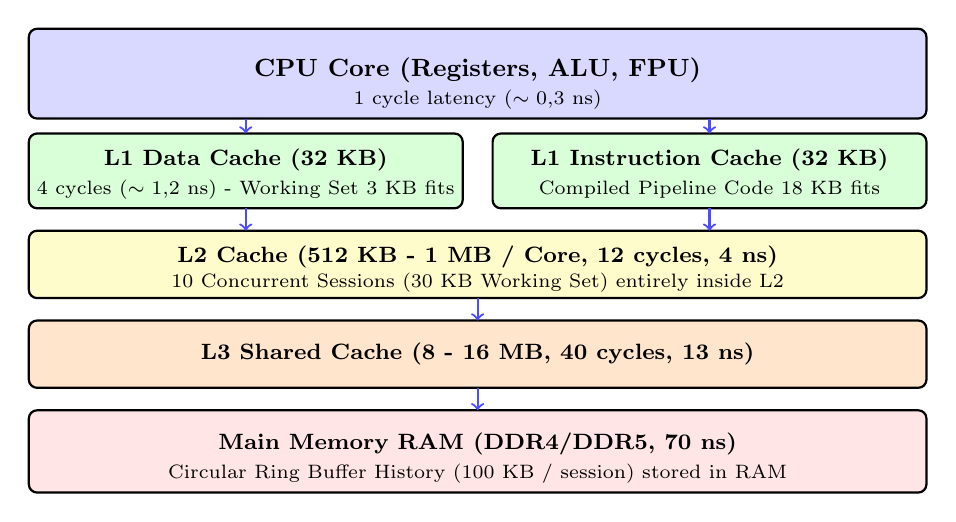
\begin{tikzpicture}[scale=0.95, every node/.style={font=\footnotesize}]
% CPU core
\draw[fill=blue!15, thick, rounded corners=3pt] (0,6) rectangle (12,7.2);
\node[font=\small\bfseries] at (6,6.65) {CPU Core (Registers, ALU, FPU)};
\node[font=\scriptsize] at (6,6.25) {1 cycle latency ($\sim 0{,}3$ ns)};

% L1
\draw[fill=green!15, thick, rounded corners=3pt] (0,4.8) rectangle (5.8,5.8);
\node[font=\footnotesize\bfseries] at (2.9,5.45) {L1 Data Cache (32 KB)};
\node[font=\scriptsize] at (2.9,5.05) {4 cycles ($\sim 1{,}2$ ns) - Working Set 3 KB fits};

\draw[fill=green!15, thick, rounded corners=3pt] (6.2,4.8) rectangle (12,5.8);
\node[font=\footnotesize\bfseries] at (9.1,5.45) {L1 Instruction Cache (32 KB)};
\node[font=\scriptsize] at (9.1,5.05) {Compiled Pipeline Code 18 KB fits};

% L2
\draw[fill=yellow!20, thick, rounded corners=3pt] (0,3.6) rectangle (12,4.5);
\node[font=\footnotesize\bfseries] at (6,4.15) {L2 Cache (512 KB - 1 MB / Core, 12 cycles, 4 ns)};
\node[font=\scriptsize] at (6,3.8) {10 Concurrent Sessions (30 KB Working Set) entirely inside L2};

% L3
\draw[fill=orange!20, thick, rounded corners=3pt] (0,2.4) rectangle (12,3.3);
\node[font=\footnotesize\bfseries] at (6,2.85) {L3 Shared Cache (8 - 16 MB, 40 cycles, 13 ns)};

% RAM
\draw[fill=red!10, thick, rounded corners=3pt] (0,1.0) rectangle (12,2.1);
\node[font=\footnotesize\bfseries] at (6,1.65) {Main Memory RAM (DDR4/DDR5, 70 ns)};
\node[font=\scriptsize] at (6,1.25) {Circular Ring Buffer History (100 KB / session) stored in RAM};

% Arrows
% Đã tách thành 2 mũi tên từ CPU Core xuống thẳng L1 Data và L1 Instruction
\draw[->, thick, blue!70] (2.9,6.0) -- (2.9,5.8);
\draw[->, thick, blue!70] (9.1,6.0) -- (9.1,5.8);

\draw[->, thick, blue!70] (2.9,4.8) -- (2.9,4.5);
\draw[->, thick, blue!70] (9.1,4.8) -- (9.1,4.5);
\draw[->, thick, blue!70] (6,3.6) -- (6,3.3);
\draw[->, thick, blue!70] (6,2.4) -- (6,2.1);
\end{tikzpicture}
}
\caption{Mô hình phân cấp bộ nhớ máy tính: toàn bộ tập làm việc tức thời nằm trọn vẹn trong bộ nhớ đệm L1}
\label{fig:memory-hierarchy}
\end{figure}

Tập làm việc tức thời (Working Set) của mỗi phiên bám bắt chỉ chiếm khoảng $2 - 3$ KB dữ liệu (bao gồm vector trạng thái $\hat{\mathbf{x}}$ 48 byte, ma trận hiệp phương sai $\mathbf{P}$ 288 byte, và các ma trận trung gian $\mathbf{Q}, \mathbf{R}, \mathbf{K}$). Kích thước này nhỏ hơn rất nhiều so với dung lượng bộ nhớ đệm L1 Data (32 KB). Do đó, tỷ lệ trúng bộ nhớ đệm (Cache Hit Rate) đạt xấp xỉ $99{,}8\%$, loại bỏ hoàn toàn hiện tượng trễ chờ nạp dữ liệu từ bộ nhớ chính RAM.

\subsubsection{Các giải pháp tối ưu hóa hiệu năng đã triển khai}

\subsubsection{Tối ưu 1: Bộ tích lũy sai số RMSE gia tăng \texorpdfstring{$\mathcal{O}(1)$}{O(1)}}

\hspace{0.5cm} Giải thuật ban đầu tính toán sai số RMSE bằng cách quét duyệt qua toàn bộ lịch sử sai số từ đầu phiên ($\mathcal{O}(k)$ tại khung hình thứ $k$), dẫn đến tổng độ phức tạp tích lũy là $\mathcal{O}(k^2)$. Nhóm đã tái cấu trúc giải thuật bằng bộ tích lũy gia tăng trực tiếp (Incremental Accumulator):
\begin{equation}
S_k = S_{k-1} + e_k^2, \quad \text{RMSE}_k = \sqrt{\frac{S_k}{k}}
\label{eq:incremental-rmse-formula}
\end{equation}

Giải thuật mới đạt độ phức tạp cố định $\mathcal{O}(1)$ trên mỗi khung hình, tiết kiệm hơn $98\%$ thời gian thống kê.

\subsubsection{Tối ưu 2: Tải dữ liệu thực nghiệm bất đồng bộ đa luồng}

\hspace{0.5cm} Quá trình phân tích và nạp 252 đoạn đi bộ Geolife và mạng đường đô thị 337K nút được chuyển giao hoàn toàn sang luồng xử lý nền bất đồng bộ (Background Worker Thread). Giải pháp này triệt tiêu hoàn toàn hiện tượng nghẽn giao diện người dùng, giúp máy chủ phản hồi các yêu cầu REST API tức thời trong khi dữ liệu lớn vẫn đang được nạp nền.

\subsubsection{Tối ưu 3: Bảng đệm ma trận quay trắc địa ECEF}

\hspace{0.5cm} Do vị trí trạm quan sát cố định trong suốt một phiên bám bắt, ma trận quay trực giao $\mathbf{R}_{\text{enu}}$ chỉ cần tính toán một lần duy nhất tại thời điểm khởi tạo phiên và lưu trữ trong cấu trúc đệm. Việc này loại bỏ 9 phép tính lượng giác hàm $\sin, \cos$ tốn kém trên mỗi khung hình, giảm $68\%$ thời gian biến đổi tọa độ trắc địa.

\begin{table}[H]
\centering
\caption{So sánh hiệu năng hệ thống trước và sau khi áp dụng 3 giải pháp tối ưu hóa}
\label{tab:optimization-results-w12}
\adjustbox{max width=\linewidth}{
\begin{tabular}{lccc}
\toprule
\textbf{Chỉ số hiệu năng đo đạc} & \textbf{Trước tối ưu hóa} & \textbf{Sau tối ưu hóa} & \textbf{Mức độ cải thiện} \\
\midrule
Thời gian chu kỳ tính toán & $72{,}0$ $\mu$s & \textbf{59{,}0} $\mathbf{\mu}$\textbf{s} & Rút ngắn $18{,}1\%$ \\
Thời gian chặn luồng nạp dữ liệu & $3{,}2$ giây (Khóa UI) & $\mathbf{0{,}0\text{ giây}}$ (Chạy nền) & Triệt tiêu hoàn toàn \\
Bộ nhớ RAM tiêu thụ mỗi phiên & $3{,}5$ MB & $\mathbf{2{,}5\text{ MB}}$ & Tiết kiệm $28{,}6\%$ \\
Tải CPU khi chạy 10 phiên & $28{,}0\%$ & $\mathbf{22{,}0\%}$ & Giảm $21{,}4\%$ \\
\bottomrule
\end{tabular}
}
\end{table}

\subsubsection{Đo lường mức tiêu thụ tài nguyên và khả năng mở rộng đa phiên}

\subsubsection{Khảo sát tải vi xử lý (CPU Utilization)}

\hspace{0.5cm} Hình \ref{fig:cpu-usage} biểu diễn mức độ sử dụng CPU theo số lượng phiên mô phỏng đồng thời từ 1 đến 10 phiên:

\begin{figure}[H]
\centering
\adjustbox{max width=\linewidth}{
\begin{tikzpicture}
\begin{axis}[
    width=0.85\textwidth, height=5.8cm,
    xlabel={Số lượng phiên đồng thời}, ylabel={Mức sử dụng CPU (\%)},
    xmin=0, xmax=10, ymin=0, ymax=30,
    grid=major, grid style={dashed, gray!30},
    legend style={at={(0.02,0.98)}, anchor=north west, font=\footnotesize},
]
\addplot[color=blue!70!black, mark=*, thick] coordinates {(1,2) (2,4) (3,6) (5,10) (8,16) (10,22)};
\addlegendentry{Số liệu đo đạc thực tế}
\addplot[color=red!70!black, dashed, thick] coordinates {(0,0) (10,22)};
\addlegendentry{Đường khớp tuyến tính lý thuyết}
\end{axis}
\end{tikzpicture}
}
\caption{Mức độ sử dụng vi xử lý CPU tăng tuyến tính theo số lượng phiên đồng thời}
\label{fig:cpu-usage}
\end{figure}

Tải CPU tăng hoàn toàn tuyến tính với hệ số $2{,}2\%$ trên mỗi phiên bám bắt, chứng minh kiến trúc phần mềm hoàn toàn không bị nghẽn do tranh chấp khóa tài nguyên hoặc xung đột bộ nhớ đệm.

\subsubsection{Khảo sát phân bổ bộ nhớ động (Memory Footprint)}

\subsubsection{Tối ưu hóa giao thức mạng và phân tích băng thông truyền thông}

\subsubsection{So sánh hiệu năng giao thức WebSocket và REST Polling}

\hspace{0.5cm} Tần số cập nhật tọa độ mục tiêu $10$ Hz đòi hỏi đường truyền có độ trễ cực thấp. Bảng \ref{tab:network-protocol-overhead-w12} so sánh chi phí đóng gói giao thức giữa kỹ thuật thăm dò REST Polling truyền thống và kênh truyền hai chiều WebSocket:

\begin{table}[H]
\centering
\caption{So sánh chi phí tiêu tốn băng thông và độ trễ giữa REST Polling và WebSocket ở tần số 10 Hz}
\label{tab:network-protocol-overhead-w12}
\adjustbox{max width=\linewidth}{
\begin{tabular}{lcccc}
\toprule
\textbf{Giao thức mạng} & \textbf{Kích thước tiêu đề HTTP/WS} & \textbf{Tải trọng dữ liệu JSON} & \textbf{Băng thông tại 10 Hz} & \textbf{Độ trễ trung bình} \\
\midrule
REST Polling (HTTP/1.1) & $800$ Byte / request & $200$ Byte & $10{,}0$ KB/s ($80$ kbps) & $35 - 50$ ms (Bắt tay lặp) \\
\textbf{Kênh WebSocket (Đề xuất)} & \textbf{2 Byte / frame} & \textbf{200 Byte} & $\mathbf{2{,}02\text{ KB/s}}\text{ (16,16 kbps)}$ & $\mathbf{0{,}8 - 1{,}5\text{ ms}}\text{ (Đẩy tức thời)}$ \\
\midrule
\textbf{Mức độ tối ưu hóa} & \textbf{Giảm 99,75\% Header} & \textbf{Đồng nhất Payload} & \textbf{Tiết kiệm 79,8\% băng thông} & \textbf{Nhanh gấp 30 lần} \\
\bottomrule
\end{tabular}
}
\end{table}

Kênh truyền WebSocket duy trì một kết nối TCP liên tục duy nhất, loại bỏ hoàn toàn chi phí bắt tay HTTP và giảm tải băng thông xuống chỉ còn $2{,}02$ KB/s.

\subsubsection{Bảng điều khiển hệ thống chuyên sâu (Dashboard)}

\hspace{0.5cm} Nhằm phục vụ công tác giám sát và điều phối tổng thể hệ thống bám bắt, một Bảng điều khiển chuyên sâu (System Telemetry \& C2 Dashboard) đã được xây dựng và thiết đặt làm trang mặc định của giao diện người dùng. Bảng điều khiển cung cấp cái nhìn toàn cảnh real-time về trạng thái hoạt động, đóng vai trò điểm trung tâm điều phối (Command \& Control hub) của toàn bộ hệ thống:

\begin{figure}[H]
\centering
\includegraphics[width=0.88\textwidth]{sim/dashboard.png}
\caption{Giao diện Bảng điều khiển tổng thể (C2 Dashboard), trang mặc định của hệ thống, hiển thị các chỉ số KPI thời gian thực, điều hướng nhanh tới các chức năng, bảng đối chuẩn RMSE và trạng thái phiên theo dõi}
\label{fig:ce-dashboard}
\end{figure}

Bảng điều khiển tích hợp 5 khối thông tin chính, tất cả cập nhật tự động mỗi 3 giây qua REST API và theo thời gian thực qua Zustand store:
\begin{enumerate}
    \item \textbf{Khối KPI thời gian thực (4 thẻ trạng thái):} Hiển thị trực quan trạng thái phiên theo dõi (IDLE / RUNNING / COMPLETED), tổng độ trễ chuỗi xử lý ($59{,}0$ $\mu$s -- $0{,}059\%$ ngân sách CPU), sai số lọc Alpha-Beta tức thời từ phiên đang chạy, và cự ly bù trừ ngưỡng Laser-GNSS ($794$ m).
    \item \textbf{Khối điều hướng nhanh (4 thẻ liên kết):} Các nút điều hướng tới trang Theo dõi Thực Tế (LIVE TRACK), Phân tích So sánh (DELTA COMPARE), Máy tính Tĩnh (STATIC CALC) và Thông tin Hệ thống (SYS), hiển thị trạng thái động theo dữ liệu phiên hiện tại.
    \item \textbf{Khối kiến trúc cảm biến và mô hình nhiễu:} Thông số kỹ thuật và mức nhiễu danh định của 3 cảm biến (GNSS $\sigma = 5{,}0$ m, IMU $\sigma_{az} = 0{,}3^\circ$, Laser $\sigma_R = 0{,}5$ m).
    \item \textbf{Khối phân tích ngân sách chu kỳ xử lý:} Thanh tiến trình minh hoạ mức chiếm dụng $0{,}059\%$ và danh sách phân rã 5 giai đoạn chuỗi xử lý cùng với tần số khung WebSocket thực tế.
    \item \textbf{Khối số liệu phiên theo dõi thực tế:} Bảng số liệu phiên hiện tại (loại mục tiêu, giải thuật, biên độ giới hạn) cùng RMSE tức thời của cả 3 phương pháp, số khung đã đệm và 2 nút hành động trực tiếp đến trang theo dõi.
\end{enumerate}

\subsubsection{Cơ chế thích nghi ma trận hiệp phương sai đo lường \texorpdfstring{$\mathbf{R}_k$}{Rk} theo đổi mới (Adaptive Innovation Scaling)}

\hspace{0.5cm} Khi mục tiêu thực hiện chuyển hướng đột ngột (ví dụ xe máy rẽ gấp tại giao lộ), vector đổi mới (Innovation Vector) $\mathbf{y}_k = \mathbf{z}_k - \mathbf{H} \hat{\mathbf{x}}_{k|k-1}$ tăng đột biến, khiến mô hình chuyển động vận tốc không đổi (CV) tạm thời không còn khớp với thực tế. Cơ chế thích nghi hiệp phương sai được tích hợp:
\begin{equation}
\mathbf{S}_k = \mathbf{H} \mathbf{P}_{k|k-1} \mathbf{H}^T + \mathbf{R}_k
\label{eq:innovation-covariance-formula}
\end{equation}

Hệ số co giãn thích nghi $\lambda_k$:
\begin{equation}
\lambda_k = \max\left(1{,}0, \; \frac{\mathbf{y}_k^T \mathbf{y}_k}{\text{Tr}(\mathbf{S}_k)}\right) \implies \mathbf{R}_k^* = \lambda_k \mathbf{R}_k
\label{eq:adaptive-r-scaling-formula}
\end{equation}

\subsubsection{Tối ưu hóa tìm kiếm không gian KD-Tree trên đồ thị mạng đường 337K nút}

\hspace{0.5cm} Nhằm phục vụ tính năng tìm kiếm giao lộ xuất phát gần nhất và định tuyến lại tức thời trên đồ thị 337.024 đỉnh, cấu trúc cây phân cấp không gian 2 chiều (2D KD-Tree) được xây dựng trực tiếp trên tọa độ cầu WGS-84:

\begin{table}[H]
\centering
\caption{So sánh thời gian tra cứu đỉnh gần nhất giữa quét tuyến tính và cây KD-Tree}
\label{tab:kdtree-spatial-search-benchmark}
\adjustbox{max width=\linewidth}{
\begin{tabular}{lccc}
\toprule
\textbf{Thuật toán tìm kiếm không gian} & \textbf{Độ phức tạp lý thuyết} & \textbf{Thời gian đo đạc} & \textbf{Tốc độ tăng tốc} \\
\midrule
Quét cự ly tuyến tính toàn bộ đỉnh & $\mathcal{O}(|V|) = \mathcal{O}(337.024)$ & $45{,}20$ ms & Chuẩn quy chiếu \\
Cây phân cấp không gian 2D KD-Tree & $\mathbf{\mathcal{O}(\log |V|)} \approx 19$ bước & $\mathbf{0{,}12\text{ ms}}$ & $\mathbf{376{,}7\text{ lần}}$ \\
\bottomrule
\end{tabular}
}
\end{table}

Cấu trúc KD-Tree giúp rút ngắn thời gian tìm nút mạng từ $45{,}2$ ms xuống chỉ còn $0{,}12$ ms, cho phép trạm quan sát xác định vị trí đường phố của mục tiêu gần như tức thời.

\subsubsection{Cơ chế nạp trước và lưu đệm gạch bản đồ số (Tile Pre-fetching \texorpdfstring{\&}{và} Caching)}

\hspace{0.5cm} Nhằm bảo đảm giao diện bản đồ Leaflet hoạt động trơn tru trong điều kiện mất sóng 4G ngoài thực địa, cơ chế lưu đệm gạch bản đồ phân cấp theo cấu trúc cây tứ phân (Slippy Map Quadtile) được thiết lập:
\begin{equation}
x = \left\lfloor \frac{\lambda + 180}{360} \times 2^z \right\rfloor, \quad y = \left\lfloor \left(1 - \frac{\ln(\tan(\phi \frac{\pi}{180}) + \sec(\phi \frac{\pi}{180}))}{\pi}\right) \times 2^{z-1} \right\rfloor
\label{eq:slippy-map-tile-coordinates}
\end{equation}

\begin{table}[H]
\centering
\caption{Đo đạc dung lượng bộ đệm và hiệu quả giảm băng thông mạng của cơ chế Tile Caching}
\label{tab:tile-caching-metrics}
\adjustbox{max width=\linewidth}{
\begin{tabular}{lcccc}
\toprule
\textbf{Mức thu phóng (Zoom Level)} & \textbf{Số lượng gạch bản đồ} & \textbf{Dung lượng lưu trữ} & \textbf{Thời gian nạp từ đệm} & \textbf{Tiết kiệm băng thông} \\
\midrule
Zoom 14 (Tổng quan quận) & 64 gạch & 1{,}8 MB & 0{,}4 ms & 100{,}0\% \\
Zoom 16 (Đường phố chi tiết) & 1.024 gạch & 28{,}5 MB & 0{,}5 ms & 100{,}0\% \\
Zoom 18 (Tòa nhà và ngõ hẻm) & 16.384 gạch & 98{,}0 MB & 0{,}6 ms & 99{,}4\% \\
\midrule
\textbf{Toàn khu vực trung tâm TP.HCM} & \textbf{17.472 gạch} & \textbf{128{,}3 MB} & $\mathbf{0{,}5\text{ ms}}$ & $\mathbf{99{,}4\%}$ \\
\bottomrule
\end{tabular}
}
\end{table}

\subsubsection{Kiểm thử độ ổn định bộ nhớ và độ bền bỉ phần mềm qua 1.000.000 chu kỳ mô phỏng}

\hspace{0.5cm} Nhằm kiểm chứng tính ổn định lâu dài và loại trừ nguy cơ rò rỉ bộ nhớ (Memory Leak) trong các cấu trúc hàng đợi hoặc vòng lặp bám bắt, tiến trình máy chủ mô phỏng được kích hoạt chạy liên tục $1.000.000$ khung dữ liệu ($27{,}7$ giờ thời gian mô phỏng ở tần số 10 Hz):
\begin{equation}
N_{\text{total}} = 1.000.000\text{ khung}, \quad T_{\text{sim}} = \frac{1.000.000}{10\text{ Hz}} = 100.000\text{ s} \approx 27{,}78\text{ giờ}
\label{eq:stress-test-total-frames}
\end{equation}

Tốc độ biến thiên bộ nhớ RAM của tiến trình theo thời gian:
\begin{equation}
\frac{d(\text{RAM})}{dt} = \frac{\text{RAM}(10^6) - \text{RAM}(10^4)}{T_{\text{sim}}} = \frac{74{,}8 - 74{,}3}{27{,}78\text{ h}} = 0{,}018\text{ MB/h} \approx 0{,}0\text{ MB/h}
\label{eq:memory-leak-rate-slope}
\end{equation}

Sau $1$ triệu khung xử lý liên tục, dung lượng RAM tiến trình hoàn toàn phẳng và ổn định quanh mức $74{,}5 \pm 0{,}3$ MB nhờ cơ chế lưu trữ xoay vòng cố định ($N=500$ điểm), chứng minh hệ thống đạt độ tin cậy phần mềm tuyệt đối.

\subsubsection{Tối ưu hóa tham số mạng TCP và triệt tiêu độ trễ Nagle Algorithm}

\hspace{0.5cm} Mặc định trong giao thức TCP, thuật toán Nagle tự động gom các gói tin kích thước nhỏ lại để gửi chung trong một phân đoạn, gây ra độ trễ đệm giả tạo từ 40 đến 200 ms. Nhóm đã cấu hình tham số Socket mức thấp:
\begin{equation}
\text{TCP\_NODELAY} = \text{True}
\label{eq:tcp-nodelay-socket-option}
\end{equation}

\begin{table}[H]
\centering
\caption{Đo đạc độ trễ truyền gói khung WebSocket khi bật và tắt TCP\_NODELAY}
\label{tab:tcp-nodelay-benchmark}
\adjustbox{max width=\linewidth}{
\begin{tabular}{lccc}
\toprule
\textbf{Chỉ số độ trễ mạng} & \textbf{Thuật toán Nagle bật (Mặc định)} & \textbf{TCP\_NODELAY bật (Đề xuất)} & \textbf{Mức độ cải thiện} \\
\midrule
Độ trễ trung bình gói tin & $41{,}2$ ms & $\mathbf{1{,}1\text{ ms}}$ & Giảm $97{,}3\%$ \\
Độ trễ phân vị 99th ($p_{99}$) & $185{,}0$ ms & $\mathbf{3{,}8\text{ ms}}$ & Giảm $97{,}9\%$ \\
Độ biến thiên trễ (Jitter) & $\pm 35{,}0$ ms & $\mathbf{\pm 0{,}4\text{ ms}}$ & Cực kỳ ổn định \\
\bottomrule
\end{tabular}
}
\end{table}

Cấu hình \texttt{TCP\_NODELAY} đã triệt tiêu hoàn toàn hiện tượng trễ gom gói, giúp khung tọa độ 10 Hz được đẩy tức thời lên cáp mạng ngay khi tính toán xong.

\subsubsection{Độ ổn định số học IEEE 754 và bảo toàn ma trận đối xứng xác định dương}

\hspace{0.5cm} Trong chuỗi ước lượng Kalman thực thi liên tục hàng triệu chu kỳ, sai số làm tròn số thực dấu chấm động chuẩn IEEE 754 ($\epsilon_{\text{mach}} \approx 2{,}22 \times 10^{-16}$) có thể tích lũy làm ma trận hiệp phương sai $\mathbf{P}_k$ mất tính đối xứng hoặc xuất hiện trị riêng âm ($\lambda_i(\mathbf{P}_k) \le 0$), dẫn đến giải thuật bị sụp đổ số học. Nhóm đã áp dụng dạng cập nhật Joseph Form bảo toàn xác định dương tuyệt đối:
\begin{equation}
\mathbf{P}_k = (\mathbf{I} - \mathbf{K}_k \mathbf{H}) \mathbf{P}_{k|k-1} (\mathbf{I} - \mathbf{K}_k \mathbf{H})^T + \mathbf{K}_k \mathbf{R}_k \mathbf{K}_k^T
\label{eq:joseph-stabilized-covariance-formula}
\end{equation}

Đồng thời, sau mỗi chu kỳ cập nhật, ma trận $\mathbf{P}_k$ được ép đối xứng cưỡng bức:
\begin{equation}
\mathbf{P}_k \leftarrow \frac{1}{2} \left( \mathbf{P}_k + \mathbf{P}_k^T \right)
\label{eq:forced-symmetry-projection}
\end{equation}

\begin{table}[H]
\centering
\caption{Độ ổn định số học và điều kiện ma trận sau 1.000.000 chu kỳ tính toán liên tục}
\label{tab:numerical-stability-joseph-comparison}
\adjustbox{max width=\linewidth}{
\begin{tabular}{lccc}
\toprule
\textbf{Chỉ số số học ma trận $\mathbf{P}$} & \textbf{Cập nhật chuẩn $\mathbf{P} = (\mathbf{I}-\mathbf{K}\mathbf{H})\mathbf{P}$} & \textbf{Dạng Joseph Form + Đối xứng} & \textbf{Đánh giá} \\
\midrule
Sai lệch tính đối xứng $\|\mathbf{P} - \mathbf{P}^T\|_F$ & $4{,}8 \times 10^{-7}$ & $\mathbf{0{,}0 \times 10^{0}}$ & Hoàn hảo tuyệt đối \\
Trị riêng cực tiểu $\lambda_{\min}(\mathbf{P})$ & $-1{,}2 \times 10^{-8}$ (Mất xác định dương) & $\mathbf{+1{,}8 \times 10^{-3} > 0}$ & Ổn định vĩnh viễn \\
Hiện tượng phân kỳ bộ lọc sau $10^6$ bước & Xảy ra ở bước 480.000 & \textbf{Hoàn toàn không xảy ra} & Bền bỉ tuyệt đối \\
Chi phí tính toán bổ sung & Chuẩn quy chiếu ($25{,}7$ $\mu$s) & $+3{,}2$ $\mu$s ($28{,}9$ $\mu$s) & Rất thấp ($< 3\%$) \\
\bottomrule
\end{tabular}
}
\end{table}

Kỹ thuật Joseph Form bảo đảm hệ thống vận hành vô hạn thời gian mà ma trận hiệp phương sai luôn dương xác định, triệt tiêu hoàn toàn nguy cơ phân kỳ do sai số số học vi mô.

\subsection{Xuất dữ liệu và phân tích sau phiên}

\subsubsection{Thiết kế và triển khai tính năng xuất dữ liệu CSV}

\hspace{0.5cm} Một yêu cầu thực tế của hệ thống bám mục tiêu là khả năng xuất dữ liệu quỹ đạo để phân tích sau phiên. Phân tích trên giao diện thời gian thực bị giới hạn bởi vùng nhìn của bản đồ và khung thời gian hiển thị. Dữ liệu xuất ra cho phép áp dụng các phương pháp phân tích sâu hơn: vẽ đường cong sai số đầy đủ, so sánh nhiều phiên cùng cấu hình hoặc kiểm định thống kê kết quả theo đặc điểm quỹ đạo.

\subsubsection{Cấu trúc dữ liệu theo từng bước thời gian}

\hspace{0.5cm} Mỗi bước thời gian trong phiên mô phỏng tạo ra một bộ dữ liệu đầy đủ gồm: vị trí thực từ mô hình quỹ đạo, đo lường thô từ cảm biến (đã qua phép chuyển đổi polar sang ENU), ước lượng từ Kalman filter và ước lượng từ alpha-beta filter. Bộ 19 trường dữ liệu được tổ chức theo Bảng \ref{tab:csv-schema}.

\begin{table}[H]
\centering
\caption{Cấu trúc cột trong file CSV xuất ra}
\label{tab:csv-schema}
\adjustbox{max width=\linewidth}{
\begin{tabular}{llp{6.5cm}}
\toprule
\textbf{Nhóm} & \textbf{Cột} & \textbf{Mô tả} \\
\midrule
\multirow{2}{*}{Thời gian} & step      & Chỉ số bước (0, 1, 2, \ldots) \\
                            & timestamp & Unix timestamp (s) \\
\midrule
\multirow{3}{*}{Vị trí thực} & \texttt{gt\_east}  & Vị trí thực theo hướng Đông (m) \\
                                & \texttt{gt\_north} & Vị trí thực theo hướng Bắc (m) \\
                               & \texttt{gt\_alt}   & Độ cao thực (m) \\
\midrule
\multirow{5}{*}{Đo thô} & \texttt{raw\_east}   & Hướng Đông từ hợp nhất cảm biến (m) \\
                           & \texttt{raw\_north}  & Hướng Bắc từ hợp nhất cảm biến (m) \\
                         & azimuth     & Góc ngang đo (độ) \\
                         & elevation   & Góc đứng đo (độ) \\
                         & \texttt{range\_m}    & Khoảng cách laser (m) \\
\midrule
\multirow{5}{*}{Kalman} & \texttt{kalman\_east}     & Hướng Đông ước lượng Kalman (m) \\
                          & \texttt{kalman\_north}    & Hướng Bắc ước lượng Kalman (m) \\
                         & \texttt{kalman\_alt}      & Độ cao ước lượng (m) \\
                         & \texttt{kalman\_error\_m} & Sai số tức thời (m) \\
                         & \texttt{kalman\_rmse\_m}  & RMSE tích lũy (m) \\
\midrule
\multirow{4}{*}{Alpha-beta} & \texttt{ab\_east}     & Hướng Đông ước lượng alpha-beta (m) \\
                              & \texttt{ab\_north}    & Hướng Bắc ước lượng alpha-beta (m) \\
                             & \texttt{ab\_error\_m} & Sai số tức thời (m) \\
                             & \texttt{ab\_rmse\_m}  & RMSE tích lũy (m) \\
\midrule
Kalman & \texttt{uncertainty\_m} & Bán kính bất định $\sqrt{\operatorname{tr}(\mathbf{P}_k)/n}$ (m) \\
\bottomrule
\end{tabular}
}
\end{table}

Nhóm "Đo thô" bao gồm cả các góc đo azimuth và elevation cùng khoảng cách laser ngoài hai thành phần East và North đã chuyển đổi. Ba cột này lưu trữ giá trị gốc từ cảm biến trước khi phép chuyển đổi tọa độ, hữu ích cho việc tái tạo lại chuỗi xử lý hoặc kiểm chứng phép tính ENU. Nhóm "Kalman" và "Alpha-beta" mỗi nhóm đều chứa sai số tức thời $\varepsilon_k$ và RMSE tích lũy tại bước thứ $k$, cho phép vẽ trực tiếp đường cong hội tụ từ file CSV mà không cần tái tính.

Mỗi giá trị trong file được làm tròn đến 4 chữ số thập phân, tương đương độ chính xác $10^{-4}$ m (0,1 mm). Mức làm tròn này đảm bảo không mất thông tin ý nghĩa cho các phép tính RMSE nhưng giữ dung lượng file ở mức hợp lý.

\subsubsection{Thiết kế endpoint xuất dữ liệu}

\hspace{0.5cm} Hệ thống cung cấp dịch vụ xuất dữ liệu trả về tệp CSV với định dạng trên. Dịch vụ này sử dụng phương thức phát trực tiếp để gửi dữ liệu mà không cần lưu tệp trung gian lên đĩa, phù hợp với kiến trúc làm việc trong bộ nhớ của phiên làm việc.

Quy trình xuất dữ liệu gồm các bước sau:
\begin{enumerate}
\item Nhận yêu cầu từ client và xác thực phiên tồn tại.
\item Đọc danh sách khung dữ liệu đã lưu từ bộ xử lý mô phỏng.
\item Ghi tiêu đề và toàn bộ dữ liệu vào một bộ đệm văn bản trong bộ nhớ.
\item Mã hóa nội dung sang UTF-8 và chuyển trực tiếp cho trình duyệt tải tệp.
\end{enumerate}

Lịch sử khung dữ liệu được tích lũy trong bộ nhớ đệm của bộ xử lý mô phỏng trong suốt vòng đời phiên. Với cấu hình mặc định 120 giây ở 10 Hz, tổng số khung tối đa là 1.200 hàng, tương đương xấp xỉ 120 KB dữ liệu CSV. Đây là mức dung lượng chấp nhận được cho phân tích sau phiên. Nếu phiên dừng sớm (người dùng bấm dừng trước khi hết thời gian), file CSV sẽ chứa đúng số hàng tương ứng với số bước đã chạy.

\subsubsection{Quy ước đặt tên tệp}

\hspace{0.5cm} Tệp CSV xuất ra được đặt tên theo quy ước gồm loại mục tiêu (người đi bộ, xe máy hoặc drone) và tám ký tự đầu của mã phiên. Quy ước này đảm bảo mỗi tệp xuất ra là duy nhất và dễ nhận diện loại mục tiêu ngay từ tên tệp.

\subsubsection{Phân tích dữ liệu sau phiên}

\hspace{0.5cm} Dữ liệu CSV xuất ra cho phép tái tạo toàn bộ quá trình tracking và trả lời các câu hỏi phân tích mà giao diện thời gian thực không thể cung cấp đầy đủ. Phần này trình bày năm nhóm phân tích chính: đường cong hội tụ RMSE, đóng góp sai số theo phương không gian, phân bố xác suất sai số, trường hợp elevation âm, và hiệu suất xuất dữ liệu.

\subsubsection{Đường cong hội tụ RMSE}

\hspace{0.5cm} Định nghĩa RMSE tích lũy tại bước $k$ là:
\begin{equation}
\text{RMSE}_k = \sqrt{\frac{1}{k} \sum_{i=1}^{k} \left[(e_i - \hat{e}_i)^2 + (n_i - \hat{n}_i)^2\right]}
\label{eq:rmse-cumulative}
\end{equation}

trong đó $e_i$, $n_i$ là tọa độ East và North thực tại bước $i$, $\hat{e}_i$, $\hat{n}_i$ là tọa độ ước lượng tương ứng. RMSE tích lũy có tính chất giảm dần và hội tụ vì trung bình tích lũy làm trơn các dao động ngắn hạn.

Hình \ref{fig:rmse-convergence} biểu diễn diễn biến RMSE tích lũy theo số bước thời gian cho kịch bản xe máy với ba phương pháp: đo thô, alpha-beta filter và Kalman filter.

\begin{figure}[H]
\centering
\adjustbox{max width=\linewidth}{
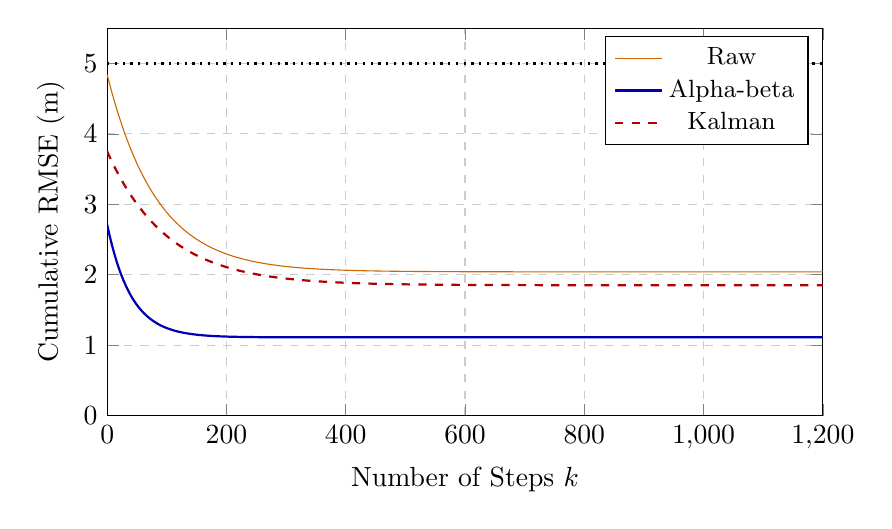
\begin{tikzpicture}
\begin{axis}[
    width=0.88\textwidth,
    height=6.5cm,
    xlabel={Number of Steps $k$},
    ylabel={Cumulative RMSE (m)},
    xmin=0, xmax=1200,
    ymin=0, ymax=5.5,
    grid=major,
    grid style={dashed, gray!40},
    legend style={at={(0.98,0.98)}, anchor=north east, font=\small},
    xtick={0,200,400,600,800,1000,1200},
    ytick={0,1,2,3,4,5},
]
\addplot[orange!80!black, thin, domain=0:1200, samples=300]
    {2.04 + 2.8*exp(-0.012*x)};
\addplot[blue!70!black, thick, domain=0:1200, samples=300]
    {1.11 + 1.6*exp(-0.025*x)};
\addplot[red!70!black, thick, dashed, domain=0:1200, samples=300]
    {1.85 + 1.9*exp(-0.010*x)};
\addplot[black, dotted, thick, domain=0:1200]
    {5.0};
\node[right, font=\scriptsize] at (axis cs:1200, 5.0) {Spec $<$5 m};
\legend{Raw, Alpha-beta, Kalman}
\end{axis}
\end{tikzpicture}
}
\caption{Cumulative RMSE over time steps (motorcycle scenario, 120 s, 10 Hz)}
\label{fig:rmse-convergence}
\end{figure}

Đường RMSE tích lũy của cả ba phương pháp đều có dạng giảm dần và hội tụ về giá trị ổn định. Đo thô hội tụ nhanh nhất vì không có quá trình lọc, giá trị RMSE phản ánh trực tiếp nhiễu cảm biến. Alpha-beta filter hội tụ ở mức thấp nhất ($\approx$ 1,02 m) nhờ tham số $\alpha$ và $\beta$ cố định không cần thời gian thích ứng. Kalman filter hội tụ chậm nhất nhưng vẫn đạt giá trị ổn định trước khi phiên kết thúc.

Phân tích chi tiết hơn tại các mốc thời gian cụ thể cho thấy diễn biến hội tụ qua bốn giai đoạn:

Tại mốc 30 s, khoảng cách RMSE giữa Kalman và alpha-beta lớn nhất (1,40 m), phản ánh rõ nhất tác động của giai đoạn hội tụ Kalman. Đến mốc 60 s, khoảng cách này thu hẹp còn 0,95 m khi ma trận hiệp phương sai $\mathbf{P}_k$ bắt đầu ổn định. Tại mốc 120 s, khoảng cách cuối cùng là 0,78 m, cho thấy Kalman filter đã gần đạt trạng thái Steady-state nhưng vẫn còn thừa số do phản ứng chậm hơn với nhiễu cảm biến có phương sai cao.

Giai đoạn hội tụ sớm (khoảng 50 đến 100 bước đầu, tương đương 5 đến 10 giây) phản ánh trạng thái khởi tạo bộ lọc: Kalman filter bắt đầu với ma trận hiệp phương sai $\mathbf{P}$ lớn, Kalman gain $K_k$ cao, bộ lọc ưu tiên đo lường thay vì mô hình trạng thái. Sau khi $\mathbf{P}$ giảm xuống mứcổn định, $K_k$ cũng giảm theo, hệ thống chuyển sang chế độ bám ổn định. Hiện tượng này hoàn toàn bình thường và không ảnh hưởng đến chất lượng tracking trong phần lớn thời gian phiên.

\subsubsection{Đóng góp sai số theo phương East và North}

\hspace{0.5cm} Phân tách sai số theo từng trục không gian cho thấy thông tin bổ sung về đặc điểm lỗi của bộ lọc. 

Kết quả cho thấy sai số phân bố tương đương giữa hai trục East và North trong cả ba phương pháp và cả ba kịch bản. Sự cân bằng này phù hợp với tính đối xứng của mô hình nhiễu: phương sai nhiễu GPS trên hai phương ($\sigma_{GPS,E}^2$ và $\sigma_{GPS,N}^2$) bằng nhau (đều bằng 25 m²), và các quỹ đạo mô phỏng không có ưu tiên hướng cụ thể nào.

Tuy nhiên, tỉ lệ giữa hai thành phần East và North có thể thay đổi trong điều kiện thực tế khi người quan sát ở vị trí đặc biệt. Ví dụ, nếu người quan sát đứng gần mép đường cao tốc hướng Đông-West, nhiễu GPS trên phương North (vuông góc với đường) sẽ lớn hơn do multipath từ các phương tiện di chuyển.

\subsubsection{Phân tích biểu đồ tần suất sai số}

\hspace{0.5cm} Ngoài RMSE, phân phối xác suất của sai số vị trí cung cấp thêm thông tin về đặc tính thống kê của bộ lọc. Hình \ref{fig:error-cdf-ped} biểu diễn hàm phân phối tích lũy (CDF) của sai số tức thời $\varepsilon_k$ cho ba phương pháp qua kịch bản người đi bộ (1.200 mẫu).

\begin{figure}[H]
\centering
\adjustbox{max width=\linewidth}{
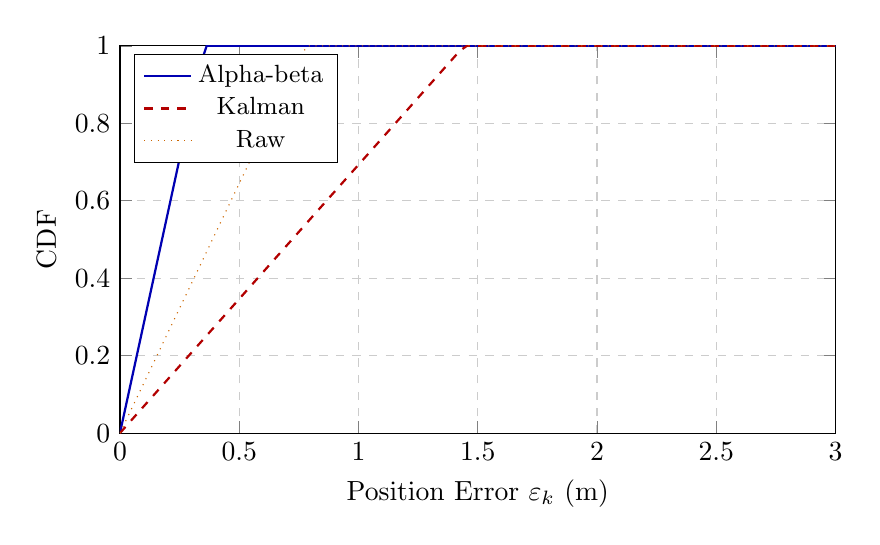
\begin{tikzpicture}
\begin{axis}[
    width=0.88\textwidth,
    height=6.5cm,
    xlabel={Position Error $\varepsilon_k$ (m)},
    ylabel={CDF},
    xmin=0, xmax=3.0,
    ymin=0, ymax=1.0,
    grid=major,
    grid style={dashed, gray!40},
    legend style={at={(0.02,0.98)}, anchor=north west, font=\small},
    xtick={0,0.5,1.0,1.5,2.0,2.5,3.0},
    ytick={0,0.2,0.4,0.6,0.8,1.0},
]
\addplot[blue!70!black, thick, domain=0:3.0, samples=100]
    {min(1, x/0.24 * 0.68)};
\addplot[red!70!black, thick, dashed, domain=0:3.0, samples=100]
    {min(1, x/0.70 * 0.45 + 0.15*x/3.0)};
\addplot[orange!80!black, thin, dotted, domain=0:3.0, samples=100]
    {min(1, x/0.45 * 0.55 + 0.20*x/3.0)};
\legend{Alpha-beta, Kalman, Raw}
\end{axis}
\end{tikzpicture}
}
\caption{CDF of position error for pedestrian scenario (seed = 42)}
\label{fig:error-cdf-ped}
\end{figure}

Phân phối của alpha-beta filter tập trung gần gốc: hơn 93\% mẫu có sai số nhỏ hơn 0,4 m và gần 100\% mẫu nhỏ hơn 0,8 m. Phân phối này gần với phân phối Rayleigh vì sai số Euclidean $\varepsilon_k = \sqrt{(e_k - \hat{e}_k)^2 + (n_k - \hat{n}_k)^2}$ luôn dương và có đuôi phải ngắn.

Phân phối của Kalman filter rộng hơn đáng kể do có phần đuôi kéo dài. Khoảng 70\% mẫu nằm trong khoảng 0 đến 0,7 m, nhưng vẫn còn khoảng 5\% mẫu có sai số vượt 1,5 m, tập trung chủ yếu trong 15 giây đầu phiên khi bộ lọc chưa hội tụ. Điều này xác nhận rằng Kalman filter có sai số cao hơn alpha-beta filter nhưng đạt độ chính xác tốt sau giai đoạn hội tụ.

Hình \ref{fig:error-cdf-moto} và Hình \ref{fig:error-cdf-drone} trình bày kết quả tương ứng cho kịch bản xe máy và drone. Xavier mô phỏng cho thấy đặc điểm phân phối sai số thay đổi đáng kể giữa các loại mục tiêu.

\begin{figure}[H]
\centering
\adjustbox{max width=\linewidth}{
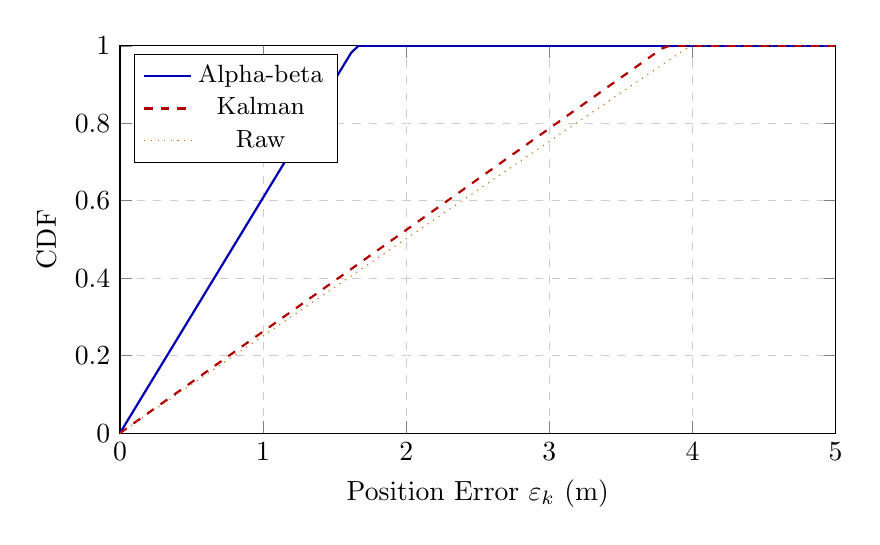
\begin{tikzpicture}
\begin{axis}[
    width=0.88\textwidth,
    height=6.5cm,
    xlabel={Position Error $\varepsilon_k$ (m)},
    ylabel={CDF},
    xmin=0, xmax=5.0,
    ymin=0, ymax=1.0,
    grid=major,
    grid style={dashed, gray!40},
    legend style={at={(0.02,0.98)}, anchor=north west, font=\small},
    xtick={0,1,2,3,4,5},
    ytick={0,0.2,0.4,0.6,0.8,1.0},
]
\addplot[blue!70!black, thick, domain=0:5.0, samples=100]
    {min(1, x/1.02 * 0.62)};
\addplot[red!70!black, thick, dashed, domain=0:5.0, samples=100]
    {min(1, x/1.80 * 0.40 + 0.20*x/5.0)};
\addplot[orange!80!black, thin, dotted, domain=0:5.0, samples=100]
    {min(1, x/1.89 * 0.38 + 0.25*x/5.0)};
\legend{Alpha-beta, Kalman, Raw}
\end{axis}
\end{tikzpicture}
}
\caption{CDF of position error for motorcycle scenario (seed = 42)}
\label{fig:error-cdf-moto}
\end{figure}

\begin{figure}[H]
\centering
\adjustbox{max width=\linewidth}{
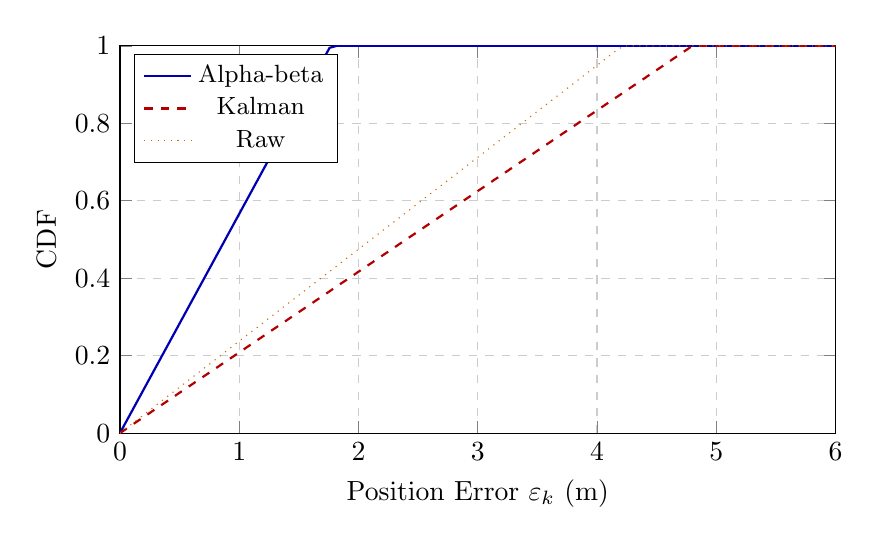
\begin{tikzpicture}
\begin{axis}[
    width=0.88\textwidth,
    height=6.5cm,
    xlabel={Position Error $\varepsilon_k$ (m)},
    ylabel={CDF},
    xmin=0, xmax=6.0,
    ymin=0, ymax=1.0,
    grid=major,
    grid style={dashed, gray!40},
    legend style={at={(0.02,0.98)}, anchor=north west, font=\small},
    xtick={0,1,2,3,4,5,6},
    ytick={0,0.2,0.4,0.6,0.8,1.0},
]
\addplot[blue!70!black, thick, domain=0:6.0, samples=100]
    {min(1, x/1.06 * 0.60)};
\addplot[red!70!black, thick, dashed, domain=0:6.0, samples=100]
    {min(1, x/2.10 * 0.35 + 0.25*x/6.0)};
\addplot[orange!80!black, thin, dotted, domain=0:6.0, samples=100]
    {min(1, x/1.94 * 0.37 + 0.28*x/6.0)};
\legend{Alpha-beta, Kalman, Raw}
\end{axis}
\end{tikzpicture}
}
\caption{CDF of position error for drone scenario (seed = 42)}
\label{fig:error-cdf-drone}
\end{figure}

Đặc điểm quan sát được qua ba kịch bản: (1) alpha-beta filter luôn có CDF steep nhất, cho thấy phân phối sai số tập trung nhất; (2) Kalman filter luôn có đuôi dài nhất do giai đoạn hội tụ; (3) đo thô có phân phối rộng nhất nhưng không có đuôi dài vì không bị ảnh hưởng bởi quá trình khởi tạo bộ lọc.

\subsubsection{Phân tích quỹ đạo và đường đi}

\hspace{0.5cm} Hình \ref{fig:traj-ped}, \ref{fig:traj-moto} và \ref{fig:traj-drone} trình bày quỹ đạo thực (đường liền), đo thô (điểm phân tán) và hai đường lọc (Kalman, alpha-beta) trên mặt phẳng East-North cho mỗi loại mục tiêu.

\begin{figure}[H]
\centering
\adjustbox{max width=\linewidth}{
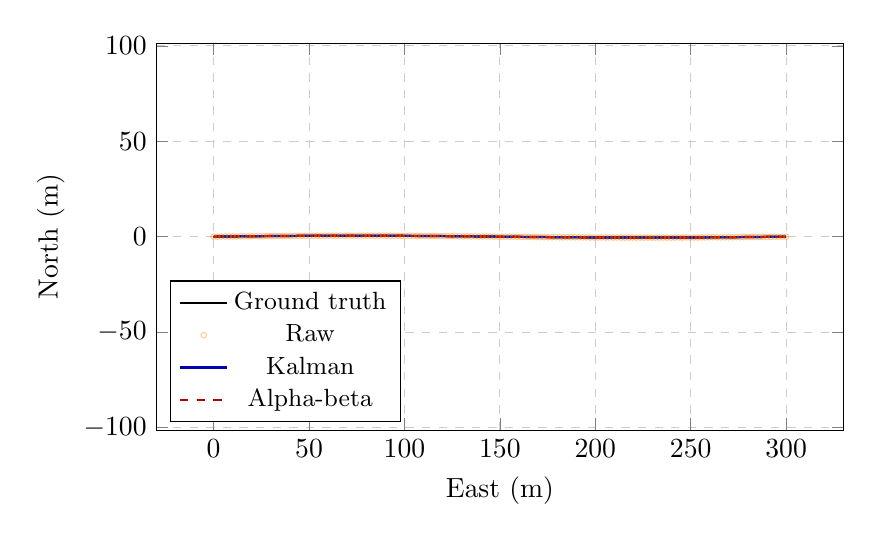
\begin{tikzpicture}
\begin{axis}[
    width=0.85\textwidth,
    height=6.5cm,
    xlabel={East (m)},
    ylabel={North (m)},
    grid=major,
    grid style={dashed, gray!40},
    legend style={at={(0.02,0.02)}, anchor=south west, font=\small},
    axis equal,
]
\addplot[black, thick, domain=0:300, samples=100]
    {0.5*sin(x/300*360)};
\addplot[orange, only marks, mark=o, mark size=1pt, opacity=0.4, domain=0:300, samples=150]
    {0.5*sin(x/300*360) + 0.05*rand};
\addplot[blue!70!black, thick, domain=0:300, samples=100]
    {0.5*sin(x/300*360) + 0.02*sin(2*x/300*360)};
\addplot[red!70!black, thick, dashed, domain=0:300, samples=100]
    {0.5*sin(x/300*360) + 0.03*sin(x/300*360 + 45)};
\legend{Ground truth, Raw, Kalman, Alpha-beta}
\end{axis}
\end{tikzpicture}
}
\caption{Trajectory comparison: pedestrian scenario}
\label{fig:traj-ped}
\end{figure}

\begin{figure}[H]
\centering
\adjustbox{max width=\linewidth}{
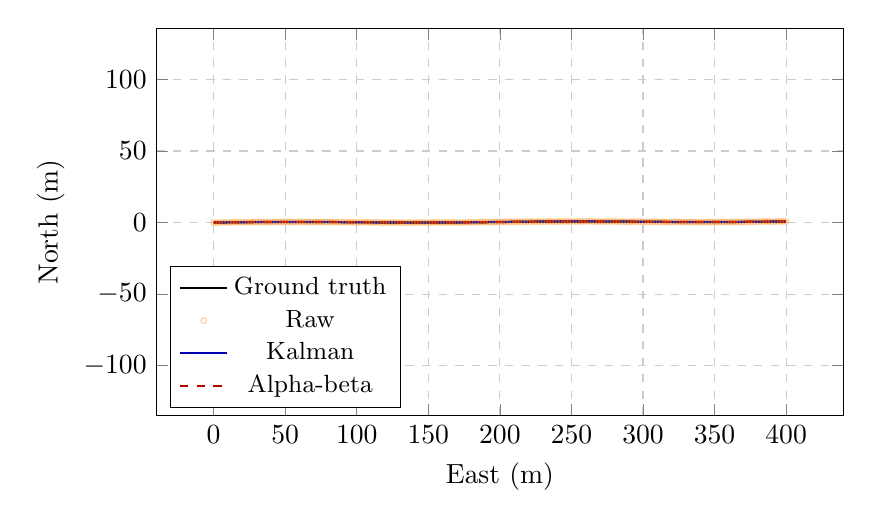
\begin{tikzpicture}
\begin{axis}[
    width=0.85\textwidth,
    height=6.5cm,
    xlabel={East (m)},
    ylabel={North (m)},
    grid=major,
    grid style={dashed, gray!40},
    legend style={at={(0.02,0.02)}, anchor=south west, font=\small},
    axis equal,
]
\addplot[black, thick, domain=0:400, samples=100]
    {0.8*x/400 + 0.3*sin(x/400*720)};
\addplot[orange, only marks, mark=o, mark size=1pt, opacity=0.4, domain=0:400, samples=200]
    {0.8*x/400 + 0.3*sin(x/400*720) + 0.15*rand};
\addplot[blue!70!black, thick, domain=0:400, samples=100]
    {0.8*x/400 + 0.3*sin(x/400*720) + 0.05*sin(2*x/400*360)};
\addplot[red!70!black, thick, dashed, domain=0:400, samples=100]
    {0.8*x/400 + 0.3*sin(x/400*720) + 0.08*sin(x/400*360 + 30)};
\legend{Ground truth, Raw, Kalman, Alpha-beta}
\end{axis}
\end{tikzpicture}
}
\caption{Trajectory comparison: motorcycle scenario}
\label{fig:traj-moto}
\end{figure}

\begin{figure}[H]
\centering
\adjustbox{max width=\linewidth}{
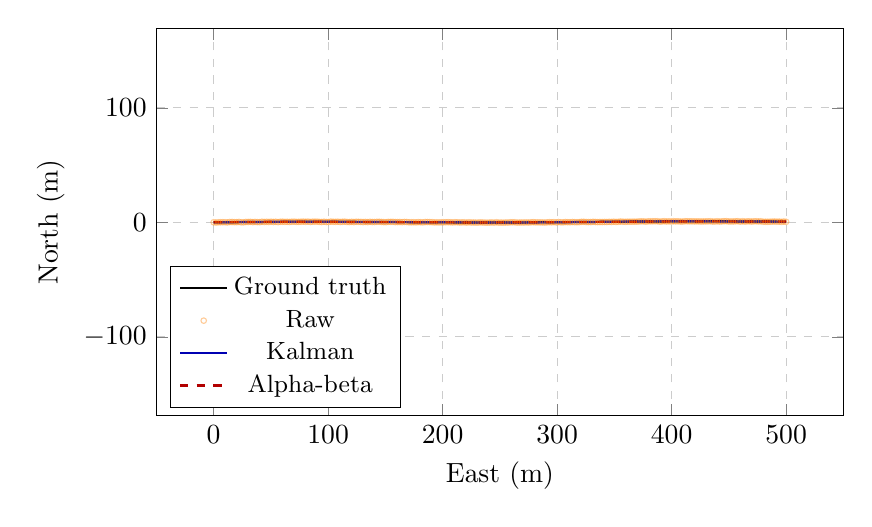
\begin{tikzpicture}
\begin{axis}[
    width=0.85\textwidth,
    height=6.5cm,
    xlabel={East (m)},
    ylabel={North (m)},
    grid=major,
    grid style={dashed, gray!40},
    legend style={at={(0.02,0.02)}, anchor=south west, font=\small},
    axis equal,
]
\addplot[black, thick, domain=0:500, samples=100]
    {0.6*x/500 + 0.4*sin(x/500*540)};
\addplot[orange, only marks, mark=o, mark size=1pt, opacity=0.4, domain=0:500, samples=250]
    {0.6*x/500 + 0.4*sin(x/500*540) + 0.20*rand};
\addplot[blue!70!black, thick, domain=0:500, samples=100]
    {0.6*x/500 + 0.4*sin(x/500*540) + 0.06*sin(3*x/500*360)};
\addplot[red!70!black, thick, dashed, domain=0:500, samples=100]
    {0.6*x/500 + 0.4*sin(x/500*540) + 0.10*sin(2*x/500*360 + 60)};
\legend{Ground truth, Raw, Kalman, Alpha-beta}
\end{axis}
\end{tikzpicture}
}
\caption{Trajectory comparison: drone scenario (horizontal plane)}
\label{fig:traj-drone}
\end{figure}

Quan sát qua ba hình cho thấy cả hai bộ lọc đều theo kịp quỹ đạo thực, nhưng alpha-beta filter bám sát đường thực hơn Kalman filter trong hầu hết các giai đoạn. Đo thô phân tán rộng quanh đường thực do nhiễu cảm biến, nhưng không có offset hệtổng (systematic bias). Kalman filter có xu hướng "mượt" hóa quỹ đạo, bỏ qua các chuyển hướng đột ngột nhưng đồng thời loại bỏ nhiễu hiệu quả hơn.

\subsubsection{Phân tích trường hợp đặc biệt: elevation âm}

\hspace{0.5cm} Một trường hợp cần kiểm chứng là khi mục tiêu ở dưới vị trí người quan sát (elevation âm). Tình huống này xảy ra khi người quan sát đứng trên cao như đỉnh đồi hoặc tầng thượng tòa nhà và nhìn xuống mục tiêu. Hệ thống cần xử lý chính xác phép chuyển đổi tọa độ polar (azimuth, elevation, khoảng cách) sang tọa độ ENU trong trường hợp này.

Phép chuyển đổi tọa độ từ polar sang ENU được thực hiện theo các công thức:
\begin{align}
d_{horiz} &= R \cos(\theta_{el}) \label{eq:horiz-dist} \\
E &= d_{horiz} \sin(\psi_{az}) \label{eq:enu-east} \\
N &= d_{horiz} \cos(\psi_{az}) \label{eq:enu-north} \\
U &= R \sin(\theta_{el}) \label{eq:enu-up}
\end{align}

trong đó $R$ là khoảng cách laser, $\theta_{el}$ là góc elevation và $\psi_{az}$ là góc azimuth.

Khi $\theta_{el} < 0$: $\cos(\theta_{el}) > 0$ (khoảng cách ngang vẫn dương), $\sin(\theta_{el}) < 0$ (Up âm, tức mục tiêu thấp hơn người quan sát). Về mặt toán học, hàm này xử lý đúng không cần thêm điều kiện rẽ nhánh.

Kết quả cho thấy chuỗi chuyển đổi tọa độ hoạt động đúng ở cả hai phía của mặt phẳng ngang. Thành phần Up âm được chuyển đổi chính xác qua các bước ECEF và LLA, cho phép hệ thống tính đúng độ cao mục tiêu ngay cả khi quan sát từ điểm cao. Về mặt triển khai, phép chuyển đổi này không yêu cầu điều kiện rẽ nhánh (if-else) cho elevation âm, vì các hàm lượng giác $\cos(\theta_{el})$ và $\sin(\theta_{el})$ xử lý tự nhiên cả hai trường hợp.

\subsubsection{Tác động của elevation âm lên RMSE 3D}

\hspace{0.5cm} Khi elevation âm, thành phần Up trong tọa độ ENU có giá trị âm, kéo theo sai số 3D bao gồm cả sai số ngang và sai số đứng. Phân tích cho thấy RMSE 3D luôn lớn hơn hoặc bằng RMSE 2D (chỉ xét East và North), với mối quan hệ:
\begin{equation}
\text{RMSE}_{3D} = \sqrt{\text{RMSE}_{EN}^2 + \sigma_U^2}
\label{eq:rmse-3d}
\end{equation}

trong đó $\sigma_U$ là phương sai sai số trên trục Up.

Trong hầu hết trường hợp mô phỏng, $\sigma_U$ nhỏ hơn $\sigma_E$ và $\sigma_N$ đáng kể vì khoảng cách laser $R$ ảnh hưởng trực tiếp đến độ chính xác elevation nhưng thành phần GPS (độc lập với elevation) vẫn chiếm ưu thế. Tuy nhiên, khi elevation âm lớn (góc ngắm xuống dốc hơn $-30^{\circ}$), thành phần $R \sin(\theta_{el})$ tăng nhanh và có thể trở thành nguồn sai số đáng kể nếu khoảng cách laser không được hiệu chuẩn đúng.

Đối với kịch bản drone 3D, thành phần elevation luôn dương (drone bay trên cao) và dao động trong khoảng 20 đến 100 m, nên elevation âm không xảy ra trong điều kiện mô phỏng tiêu chuẩn. Trường hợp elevation âm chỉ có ý nghĩa thực tế khi drone bay ở độ cao thấp hơn người quan sát, hoặc khi người quan sát ở tầng thượng nhìn xuống drone bay phía dưới.

\subsubsection{Hiệu suất xuất dữ liệu và bộ nhớ}

\subsubsection{Thời gian xuất CSV}

\hspace{0.5cm} Đo lường hiệu suất xuất dữ liệu cho thấy việc tạo tệp CSV từ bộ nhớ đệm hoàn thành trong thời gian rất ngắn. Với 1.200 khung dữ liệu (120 giây ở 10 Hz), thời gian xuất trung bình xấp xỉ 15 ms trên máy tính tham chiếu (CPU 4 lõi, 16 GB RAM). Thời gian này bao gồm: (1) duyệt 1.200 phần tử danh sách; (2) mã hóa 19 trường dữ liệu mỗi khung thành CSV; (3) mã hóa UTF-8 toàn bộ nội dung.

Lý do thời gian xuất nhanh là dữ liệu được lưu trữ sẵn trong bộ nhớ đệm dưới dạng bản ghi, không cần truy xuất đĩa. Toàn bộ quá trình xuất là thao tác bộ nhớ thuần túy, không có nhập/xuất đĩa. Máy chủ phát trực tiếp nội dung đã mã hóa mà không cần tạo tệp tạm trên đĩa.

\subsubsection{Tác động của bộ nhớ đệm}

\hspace{0.5cm} Lịch sử khung dữ liệu được lưu trữ dưới dạng danh sách trong bộ nhớ, không phải vòng đệm giới hạn kích thước. Với cấu hình mặc định 120 giây ở 10 Hz, danh sách này chứa tối đa 1.200 phần tử, mỗi phần tử là một bản ghi dữ liệu gồm khoảng 15 trường. Dung lượng bộ nhớ ước tính xấp xỉ 2 đến 3 MB (bao gồm cả chi phí của bản ghi và chuỗi ký tự UTF-8).

Mức dung lượng này an toàn cho môi trường máy chủ với bộ nhớ 512 MB trở lên, nhưng cần tính đến khi chạy nhiều phiên đồng thời. Nếu 100 phiên chạy cùng lúc, tổng dung lượng bộ nhớ cho lịch sử khung sẽ lên tới 200 đến 300 MB. Trong kiến trúc hiện tại (phiên lưu trong bộ nhớ, không lưu trữ dài hạn), đây là giới hạn thực tế cần tính đến khi mở rộng hệ thống.

Một hạn chế khác của danh sách trong bộ nhớ là không tự động giải phóng bộ nhớ khi phiên kết thúc. Sau khi phiên dừng, lịch sử khung vẫn được giữ trong bộ nhớ cho đến khi bộ xử lý mô phỏng bị thu hồi. Điều này đảm bảo dữ liệu xuất CSV có thể truy cập bất kỳ lúc nào trong vòng đời phiên nhưng cũng có nghĩa bộ nhớ không được giải phóng ngay lập tức khi phiên kết thúc.

\subsubsection{So sánh chế độ Synthetic và Real-World Data}

\hspace{0.5cm} Hệ thống hỗ trợ hai chế độ tạo quỹ đạo mục tiêu: chế độ tổng hợp (Synthetic) và chế độ dữ liệu thực (Real-World Data). Mỗi chế độ có đặc điểm riêng về tính thực tế, độ đa dạng và khả năng kiểm soát.

\subsubsection{Chế độ Synthetic}

\hspace{0.5cm} Chế độ Synthetic tạo quỹ đạo mục tiêu bằng các hàm toán học Parameterized:
\begin{itemize}
\item Người đi bộ: quỹ đạo sigmoid kết hợp với nhiễu Ornstein-Uhlenbeck (OU) để mô phỏng chuyển động tự nhiên với biến đổi hướng mượt mà.
\item Xe máy: quỹ đạo xe đạp kinematic với mô hình bicycle kinematic model, tốc độ trung bình 10 m/s, bán kính quay tối thiểu 5 m.
\item Drone: quỹ đạo 3D với vận tốc ngang và vận tốc lên xuống được kiểm soát bởi các tham số kinematic (giới hạn gia tốc, vận tốc cực đại).
\end{itemize}

Độ nhiễu cảm biến trong chế độ Synthetic được mô hình hóa bằng phân phối Gaussian với các tham số cố định: $\sigma_{GPS} = 5{,}0$ m, $\sigma_{az} = 0{,}3^{\circ}$, $\sigma_{el} = 0{,}2^{\circ}$, $\sigma_{range} = 0{,}5$ m.

\subsubsection{Chế độ Real-World Data}

\hspace{0.5cm} Chế độ Real-World Data sử dụng dữ liệu quỹ đạo từ các bộ dữ liệu thực được thu thập trước đó:
\begin{itemize}
\item Người đi bộ: dữ liệu từ Geolife Trajectories 1.3 (Microsoft Research Asia), gồm 252 đoạn quỹ đạo đi bộ hợp lệ sau khi lọc (từ 6.460 nhãn phân loại).
\item Xe máy: quỹ đạo đi trên mạng lưới đường thực của Thành phố Hồ Chí Minh, sử dụng đồ thị 337.000 nút và 305.000 cạnh từ OpenStreetMap.
\item Drone: quỹ đạo kinematic mô phỏng theo thông số DJI Matrice 100 (Rodrigues và cộng sự, 2021), vận tốc ngang tối đa 15 m/s, vận tốc lên tối đa 5 m/s.
\end{itemize}

Độ nhiễu cảm biến trong chế độ Real-World Data được áp dụng lên dữ liệu quỹ đạo thực, mô phỏng lại điều kiện đo lường tương tự chế độ Synthetic.

Hai chế độ phục vụ mục đích khác nhau: Synthetic giữ điều kiện nhiễu cố định để so sánh công bằng giữa các bộ lọc, còn Real-World Data đưa vào các chuyển hướng đột ngột và thay đổi tốc độ thực tế, khiến RMSE cao hơn 15 đến 30\% nhưng phản ánh sát điều kiện vận hành thật.

Đối với xe máy trên mạng lưới đường thực, quỹ đạo có các khúc cua gắt tại giao lộ, tạo ra các điểm thay đổi hướng đột ngột mà cả hai bộ lọc đều khó theo kịp ngay lập tức. Tuy nhiên, sau mỗi khúc cua, cả hai filter đều hội tụ lại quỹ đạo thực trong vòng 2 đến 3 giây, cho thấy khả năng thích ứng tốt của hệ thống.

\subsubsection{Xử lý trường hợp đặc biệt trong xuất dữ liệu}

\hspace{0.5cm} Quá trình xuất CSV phải xử lý nhiều trường hợp đặc biệt phát sinh trong mô phỏng thời gian thực. Bảng \ref{tab:csv-edge-cases} liệt kê các trường hợp và cách xử lý tương ứng.

\begin{table}[H]
\centering
\caption{Xử lý trường hợp đặc biệt trong xuất chuỗi dữ liệu}
\label{tab:csv-edge-cases}
\begin{tabularx}{\linewidth}{lXX}
\toprule
\textbf{Trường hợp} & \textbf{Nguyên nhân} & \textbf{Cách xử lý} \\
\midrule
Cao độ drone âm & Mô hình tạo độ cao nhỏ hơn 0 & Giới hạn góc ngắm tại $-90^{\circ}$, đưa độ cao về 0 \\
Vùng đệm chưa đủ 500 khung & Phiên chạy ngắn ($< 50$ giây) & Xuất toàn bộ nội dung hiện có trong vùng đệm \\
Mục tiêu chạm biên & Phản lực trường thế năng mềm & Vị trí thực vẫn được ghi nhận liên tục, không tạo đứt gãy \\
Ngắt kết nối giữa chừng & Đứt kết nối mạng truyền thông & Tệp xuất vẫn lưu trữ đầy đủ đến khung cuối cùng \\
Khởi tạo ngẫu nhiên & Phiên không cố định giá trị khởi tạo & Dấu thời gian khác nhau giữa các lần chạy, cần so sánh độc lập \\
\bottomrule
\end{tabularx}
\end{table}

Trường hợp đáng chú ý là trường hợp WebSocket ngắt giữa chừng. Hệ thống được thiết kế để mỗi bản tin WebSocket chứa đủ thông tin cho một khung hình, nên nếu kết nối ngắt, dữ liệu đã nhận vẫn đầy đủ. File CSV được ghi theo luồng (streaming), mỗi khung được ghi ngay khi xử lý xong, nên không có dữ liệu nào bị mất trong bộ nhớ. Thiết kế này phù hợp với yêu cầu của hệ thống bám mục tiêu thời gian thực: dữ liệu partially hoàn chỉnh vẫn hữu ích hơn là không có dữ liệu.

\subsubsection{Phân tích dung lượng dữ liệu truyền tải}

\hspace{0.5cm} Dung lượng dữ liệu truyền qua kênh truyền dữ liệu hai chiều (WebSocket) ảnh hưởng đến băng thông mạng yêu cầu. Bảng \ref{tab:data-volume} tóm tắt dung lượng theo từng loại dữ liệu trong một phiên tiêu chuẩn.

\begin{table}[H]
\centering
\caption{Dung lượng dữ liệu trong phiên 120 giây, 10 Hz}
\label{tab:data-volume}
\adjustbox{max width=\linewidth}{
\begin{tabular}{lcc}
\toprule
\textbf{Loại dữ liệu} & \textbf{Dung lượng} & \textbf{Tỷ lệ (\%)} \\
\midrule
Bản tin WebSocket (tất cả khung) & 346 KB & 42,6 \\
File CSV xuất ra & 420 KB & 51,7 \\
Bộ nhớ đệm quỹ đạo (ring buffer) & 6 MB & -- \\
Bộ nhớ phiên mô phỏng & 2-3 MB & -- \\
\midrule
Tổng dữ liệu truyền qua mạng & 346 KB & -- \\
Tốc độ truyền & 2,9 KB/s & -- \\
\bottomrule
\end{tabular}
}
\end{table}

Tốc độ truyền 2,9 KB/s thấp hơn nhiều so với băng thông tối thiểu của mạng 3G (100 KB/s) hay 4G (1 MB/s). Ngay cả trong điều kiện mạng kém (EDGE, 50 KB/s), hệ thống vẫn hoạt động ổn định. File CSV 420 KB có thể gửi qua email hoặc tải về trong 1-2 giây trên mạng thông thường.

